% !TEX program = xelatex
% !TEX encoding = UTF-8
%% ===========================================================================
%%  Mesh Registration from Scan-Derived 3D Data
%%  Internship report -- Forschungszentrum Juelich (IAS-7), July-Sept. 2026
%%  Khaoula Jellal
%%
%%  Build (XeLaTeX, Calibri 12 pt; falls back to the metric-identical Carlito):
%%     xelatex main && bibtex main && xelatex main && xelatex main
%% ===========================================================================
\documentclass[12pt,a4paper,toc=listof,toc=bibliography]{scrartcl}

\usepackage{style/report}
\usepackage{tikz}
\usetikzlibrary{arrows.meta,positioning,calc,fit}
\usepackage{pgfplots}\pgfplotsset{compat=1.16}

\usepackage[numbers,sort&compress]{natbib}
\bibliographystyle{unsrtnat}
\setlength{\bibsep}{0pt}
% DOIs as plain text (the default \Url math-mode formatting clashes with the maths font)
\newcommand{\doi}[1]{doi:~#1}

\hypersetup{
  pdftitle={Mesh Registration from Scan-Derived 3D Data: Correspondence and Optimization in Articulated Parametric Models},
  pdfauthor={Khaoula Jellal}
}

% ===========================================================================
%  FINDINGS LEDGER: each load-bearing result is declared once and cited
%  anywhere as \F{F1}; Table~\ref{tab:findings} builds itself.
% ===========================================================================
\begin{document}

% Front cover: full-bleed design (scan point cloud -> fitted model), no page number
\begin{titlepage}
\thispagestyle{empty}
\definecolor{covnavy}{HTML}{081C2A}
\definecolor{covblue}{HTML}{14506B}
\definecolor{covcyan}{HTML}{7FD6E8}
\definecolor{covgold}{HTML}{E2B04A}
\pgfmathsetseed{11}
\begin{tikzpicture}[remember picture,overlay,every node/.style={inner sep=0pt}]
  % ---- background -------------------------------------------------------
  \shade[top color=covblue!85!covnavy,bottom color=covnavy]
    (current page.south west) rectangle (current page.north east);
  % soft glow behind the model (stacked, very low opacity)
  \foreach \k in {1,...,16}{
    \fill[covcyan!60!covblue,opacity=0.028]
      ([xshift=10.5cm,yshift=12.5cm]current page.south west) ellipse ({11.5cm-\k*0.55cm} and {5.6cm-\k*0.27cm});
  }

  % ---- scan point cloud (left) resolving into the mesh (right) ------------
  \foreach \i in {1,...,330}{
    \pgfmathsetmacro{\px}{rnd*17.5+1.8}
    \pgfmathsetmacro{\py}{12.5+(rnd-0.5)*8.4}
    \pgfmathsetmacro{\o}{0.55*(1-\px/19.5)+0.04}
    \pgfmathsetmacro{\r}{0.035+0.04*rnd}
    \fill[covcyan,opacity=\o] ([xshift=\px cm,yshift=\py cm]current page.south west) circle (\r cm);
  }
  % ---- fitted ant ---------------------------------------------------------
  \node[opacity=0.97] at ([xshift=10.9cm,yshift=12.5cm]current page.south west)
    {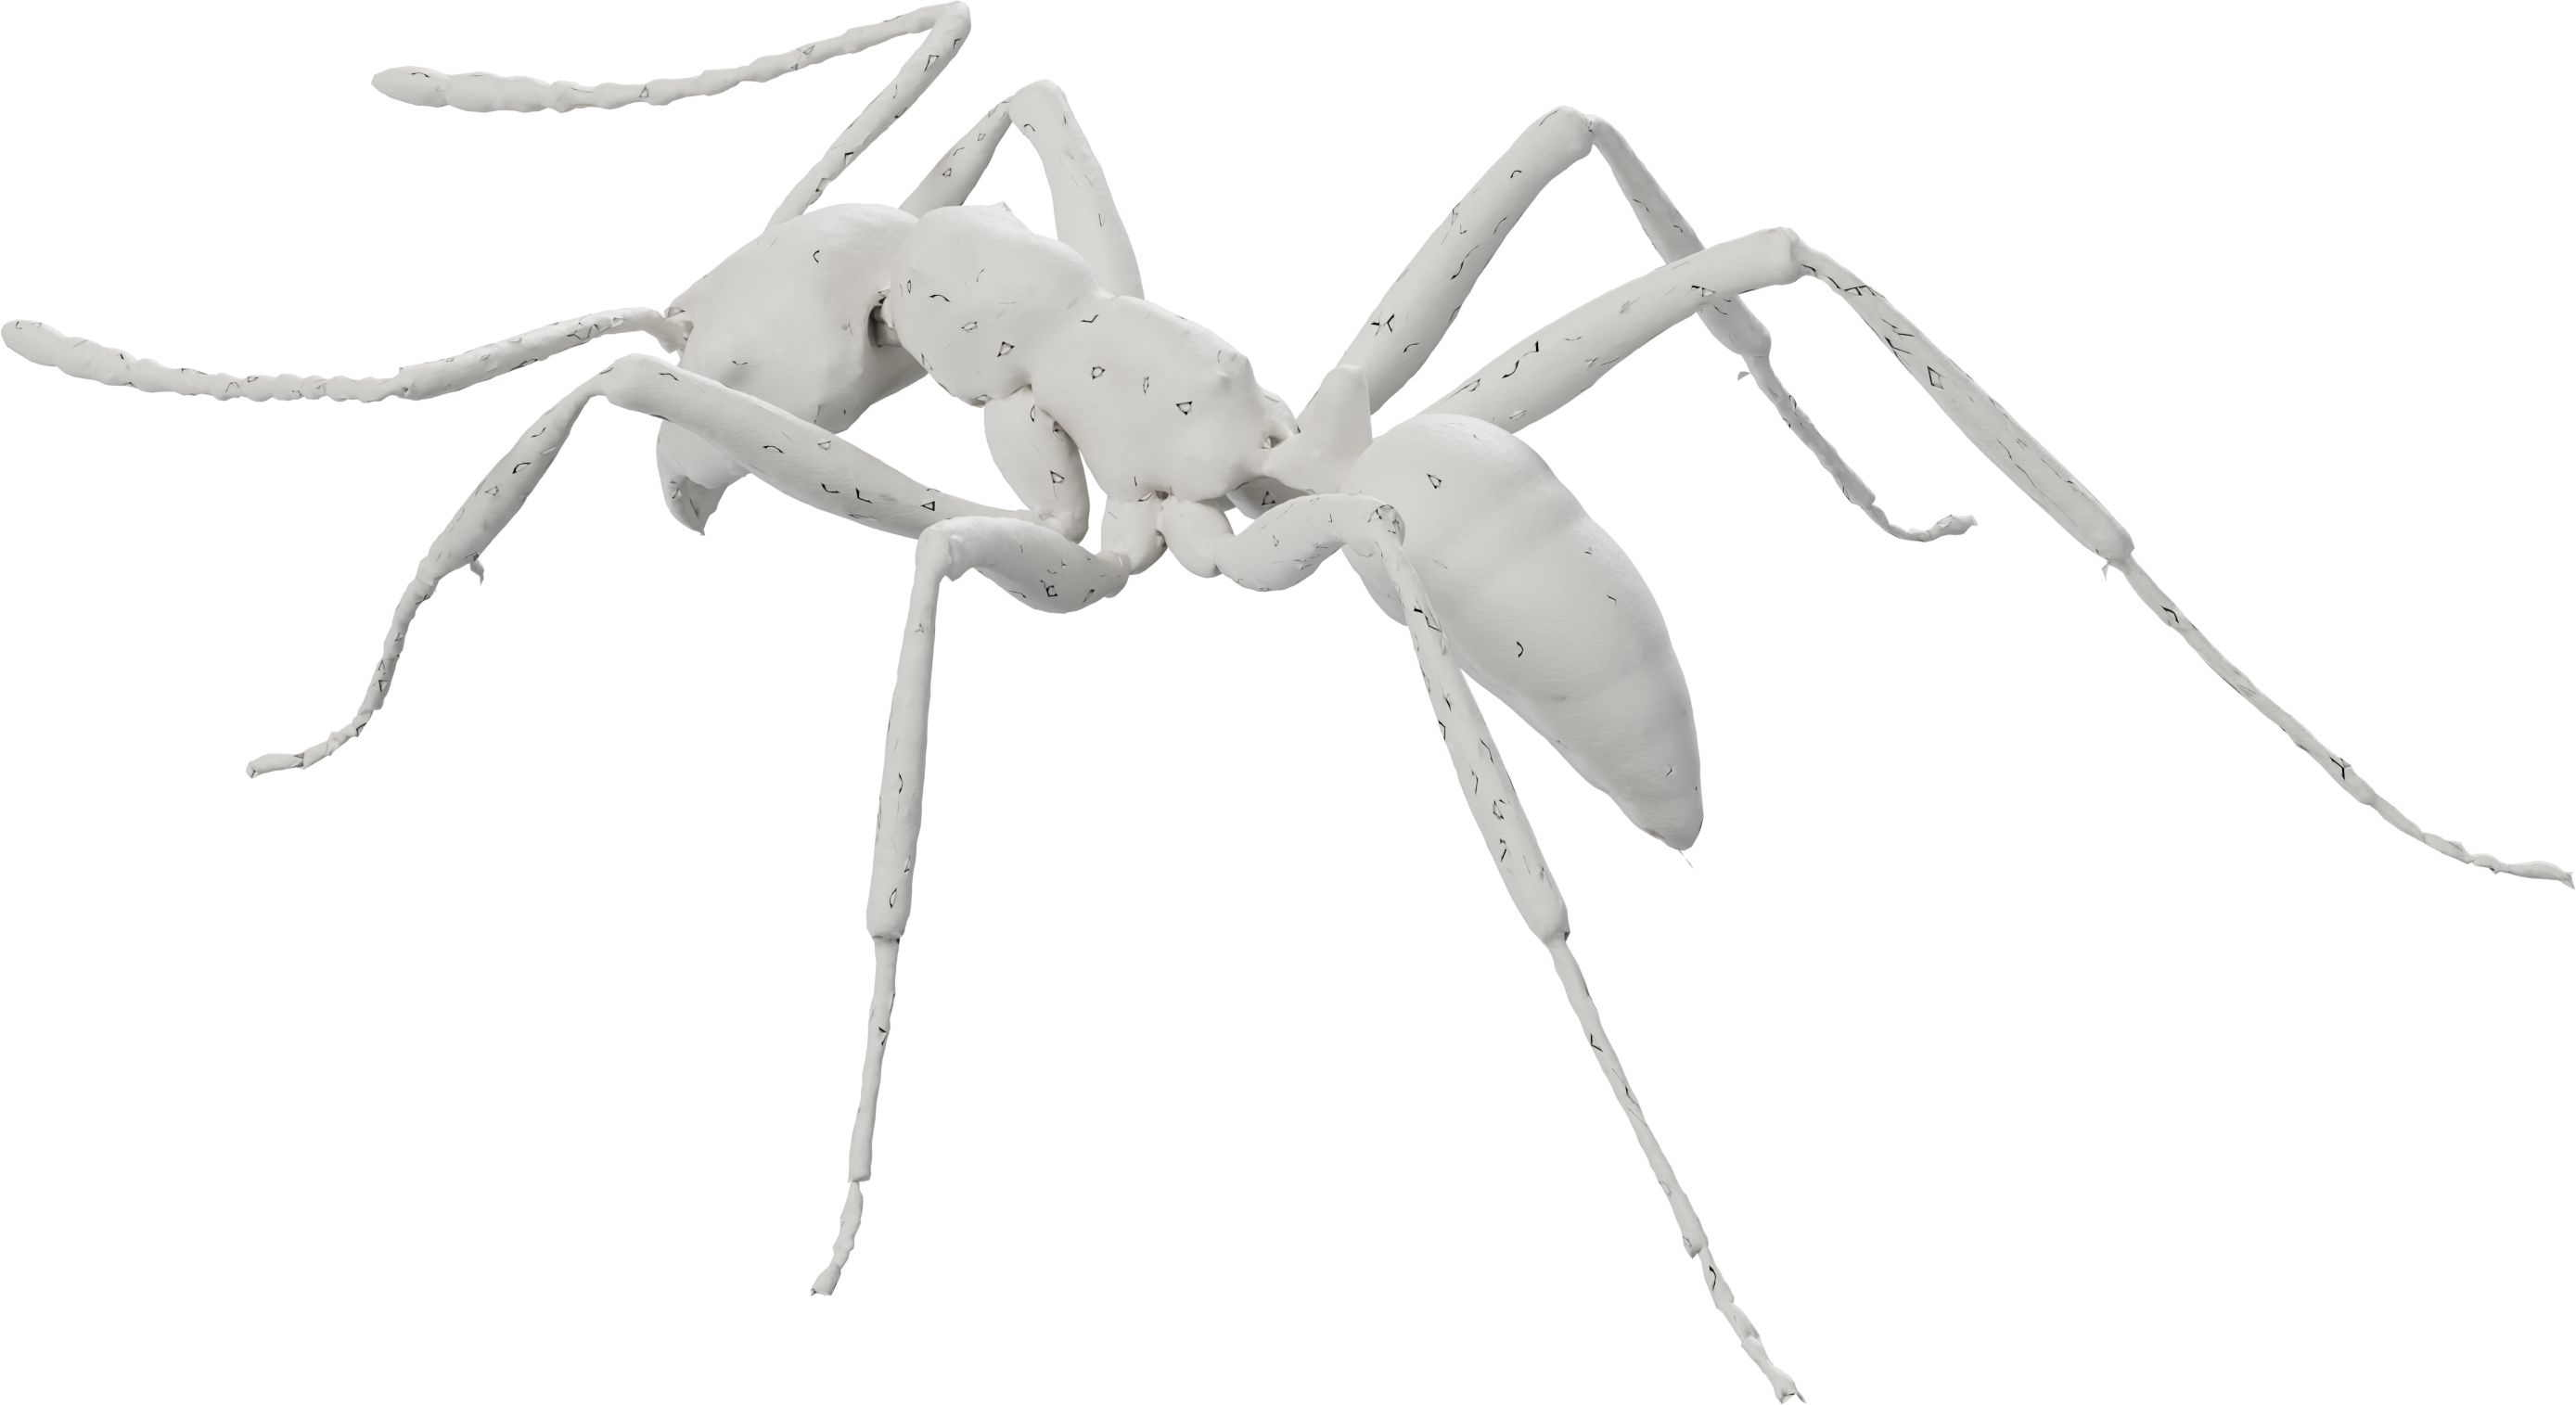
\includegraphics[width=18.6cm]{figures/cover_ant.png}};
  % correspondence ticks between scan points and model
  \foreach \a/\b/\c/\d in {3.2/14.2/6.0/13.6, 3.7/11.6/6.4/12.2, 4.8/15.5/7.4/14.6, 4.2/10.2/6.8/11.4}{
    \draw[covgold,opacity=0.75,line width=0.5pt,dash pattern=on 2pt off 2pt]
      ([xshift=\a cm,yshift=\b cm]current page.south west) --
      ([xshift=\c cm,yshift=\d cm]current page.south west);
    \fill[covgold] ([xshift=\a cm,yshift=\b cm]current page.south west) circle (0.07cm);
  }

  % ---- logos -------------------------------------------------------------
  \node[anchor=north west] at ([xshift=1.8cm,yshift=-1.3cm]current page.north west)
    {
\includegraphics[height=1.85cm]{figures/logos/juelich_white.png}};
  \node[anchor=north east] at ([xshift=-1.8cm,yshift=-1.2cm]current page.north east)
    {
\includegraphics[height=2.1cm]{figures/logos/coc_white.png}};
  \draw[covcyan,opacity=0.45,line width=0.4pt]
    ([xshift=1.8cm,yshift=-3.75cm]current page.north west) --
    ([xshift=-1.8cm,yshift=-3.75cm]current page.north east);
  \node[anchor=north west,text=covcyan,font=\small\bfseries,text width=17cm]
    at ([xshift=1.8cm,yshift=-4.1cm]current page.north west)
    {FORSCHUNGSZENTRUM J\"ULICH \;$\cdot$\; IAS-7 CIVIL SAFETY RESEARCH};
  \node[anchor=north west,text=white,opacity=0.8,font=\small,text width=17cm]
    at ([xshift=1.8cm,yshift=-4.7cm]current page.north west)
    {College of Computing -- UM6P \;$\cdot$\; Internship report};

  % ---- title --------------------------------------------------------------
  \fill[covgold] ([xshift=1.8cm,yshift=-6.0cm]current page.north west) rectangle ++(0.13cm,-4.7cm);
  \node[anchor=north west,text=white,font=\fontsize{46}{50}\selectfont\bfseries,text width=17cm]
    at ([xshift=2.45cm,yshift=-5.95cm]current page.north west) {Mesh Registration};
  \node[anchor=north west,text=white,font=\fontsize{29}{34}\selectfont,text width=17cm]
    at ([xshift=2.45cm,yshift=-7.85cm]current page.north west) {from Scan-Derived 3D Data};
  \node[anchor=north west,text=covcyan,font=\fontsize{15}{20}\selectfont\itshape,text width=16cm]
    at ([xshift=2.45cm,yshift=-9.2cm]current page.north west)
    {Correspondence and optimization in articulated\\ parametric models of insects};

  % ---- author block (right) ------------------------------------------------
  \fill[covgold] ([xshift=-1.8cm,yshift=7.0cm]current page.south east) rectangle ++(-2.6cm,0.09cm);
  \node[anchor=north east,text=white,font=\fontsize{22}{26}\selectfont\bfseries,align=right]
    at ([xshift=-1.8cm,yshift=6.75cm]current page.south east) {Khaoula Jellal};
  \node[anchor=north east,align=right,text width=9cm,font=\normalsize]
    at ([xshift=-1.8cm,yshift=5.5cm]current page.south east)
    {{\footnotesize\bfseries\color{covcyan}COMPANY SUPERVISOR}\\ \textcolor{white}{Dr.\ Fabian Plum}\\[7pt]
     {\footnotesize\bfseries\color{covcyan}ACADEMIC SUPERVISOR}\\ \textcolor{white}{Prof.\ Ayoub Arraji}\\[7pt]
     {\footnotesize\bfseries\color{covcyan}INTERNSHIP PERIOD}\\ \textcolor{white}{1 July -- 25 September 2026}};
  \node[anchor=south west,text=white,opacity=0.6,font=\footnotesize]
    at ([xshift=1.8cm,yshift=1.3cm]current page.south west) {October 2026};
\end{tikzpicture}
\end{titlepage}


\clearpage
% Abstract (English only), placed after the front cover
\thispagestyle{plain}
\section*{Abstract}
\addcontentsline{toc}{section}{Abstract}

Articulated parametric mesh models provide a shared coordinate system in
which otherwise unrelated three-dimensional scans can be compared, but
fitting them to imperfect scan-derived geometry is an ill-constrained inverse
problem: the optimiser recovers shape, pose, scale and deformation from
surface observations alone, and anatomical correspondence is an intended
consequence of those parameters rather than an independently observed
quantity. This report investigates that problem for an insect-focused
instance of the SMAL/SMPL family of models (SMILify), across defect-aware mesh
preprocessing, anatomical structural priors, learned pose initialisation,
sampling and robust optimisation, learned correspondence descriptors, and the
registration objective itself. It uses a synthetic round-trip benchmark with
exact vertex-identity ground truth and an independently annotated,
coordinate-corrected expert benchmark (11 specimens, 396 fits). The central
technical finding is that surface agreement, anatomical correspondence,
parameter recovery and measurement validity are distinct properties that do
not track one another: a fit can score a lower surface-distance loss while its
skeleton is anatomically worse; a locally accurate learned correspondence
descriptor can collapse when deployed as a dense, globally consistent field, whereas a
template-embedding head with a cycle-consistency filter can be consumed by the fitter
without ground truth;
and a measurement such as head width can agree with an independent reference
even where individual-level correspondence is not reliable enough for
specimen-by-specimen comparison. The contribution is a diagnostic and
evaluation framework (synthetic and expert ground truth, counterfactual
interventions, an adversarial metric test, and a multi-level evidence
hierarchy), together with the algorithmic and systems extensions evaluated
against it, that localises where the current pipeline loses anatomical
information and what is required before a registration can be trusted as a
biological measurement.

\medskip
\noindent\textbf{Keywords:} 3D computer vision; mesh registration; articulated
reconstruction; geometric learning; point clouds; correspondence;
differentiable optimisation; morphometric measurement.


\clearpage
{\linespread{0.82}\setlength{\parskip}{0pt}\tableofcontents}
\clearpage
\listoffigures
\vspace{1.5em}
\listoftables
\clearpage

\section{Introduction}
\label{sec:intro}

\subsection{Motivation and the failure that defined the question}

Ant scans can turn specimens that are difficult to measure repeatedly into a
source of comparable three-dimensional traits. If every scan is registered to a
common parametric model, quantities such as head width, Weber's length or
appendage proportions can be extracted systematically instead of by hand under
a microscope, which opens a route to studying morphological diversity at
population scale; recent work on \emph{Atta} workers already shows that a 3D
shape space can reveal structure that size scaling alone does not~\cite{imirzian}.
Real scans, however, whether from scAnt photogrammetry~\cite{scant} or
micro-CT, are far from ideal inputs: they contain holes, self-intersections,
arbitrary orientation and missing surface exactly at the thin structures of
greatest anatomical interest (Figure~\ref{fig:raw-scans}).

\begin{figure}[!htb]
\centering
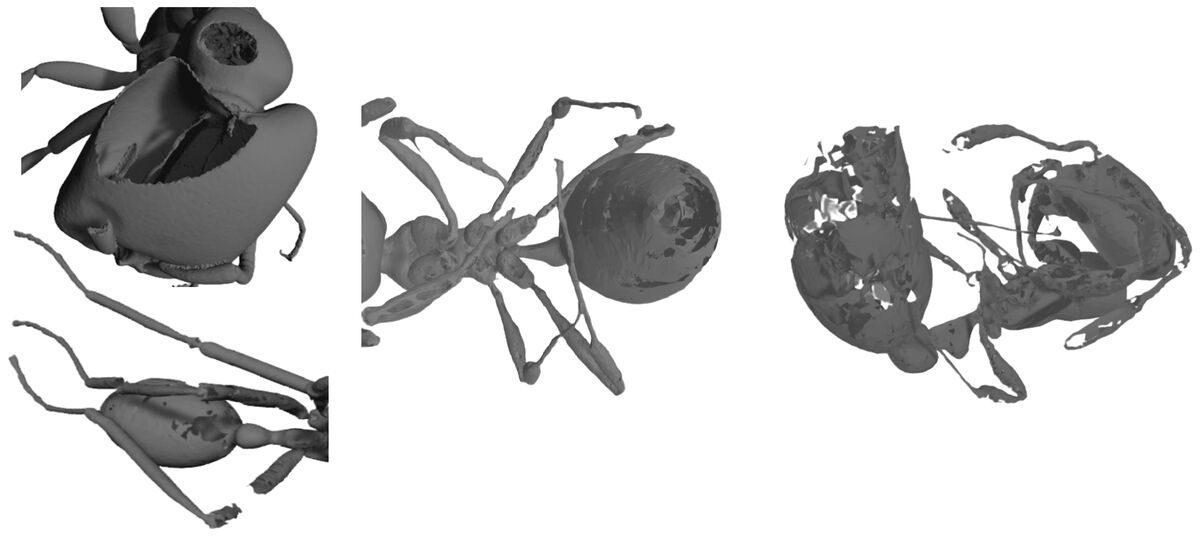
\includegraphics[width=0.50\linewidth]{figures/fig_before_registration.jpg}
\caption[Raw scans before registration]{Raw scans before registration: holes,
self-intersections and missing surface at the structures of greatest
anatomical interest.}
\label{fig:raw-scans}
\end{figure}

In the first week of July 2026, ten preprocessed ant scans were passed through
the registration pipeline. All ten optimisations converged cleanly: the loss
curves showed no divergence and the objective decreased as expected. Four of
the resulting models were nevertheless not recognisable as anatomically
meaningful ants. Legs had collapsed into the gaster and, in some fits, the head
had been absorbed into the thorax. More troublingly, several of these wrong
fits reached a \emph{lower} loss than the runs that had visibly succeeded. The
optimiser had succeeded; the registration had failed. The objective is a
symmetric point-to-point distance between two surfaces: it measures whether the
fitted mesh \emph{covers} the target, not whether vertex $i$ of the template has
landed on the anatomical point it is defined to represent. When the two
diverge, nothing in the pipeline's own numerical output signals it. This
discrepancy is the starting point of the work.

\subsection{Problem formulation: recovering a latent anatomical explanation}
\label{sec:problem}

SMILify~\cite{smilify} extends the optimisation-based SMALify
procedure~\cite{smalify} for the SMAL quadruped model~\cite{smal} to arbitrary
rigged templates, with SMIL (Skinned Multi-Insect Linear) as its insect
instance. Registration recovers, for a scan $T$, the latent variables of a
parametric mesh $M$: shape $\bm\beta$, articulated pose $\bm\theta$, scale $s$
and residual per-vertex deformation $\mathbf d$,
\begin{equation}
(\hat{\bm\beta},\hat{\bm\theta},\hat s,\hat{\mathbf d})
 =\arg\min_{\bm\beta,\bm\theta,s,\mathbf d}\;
 \mathcal{L}\big(M(\bm\beta,\bm\theta,s,\mathbf d),\,T\big).
\label{eq:registration}
\end{equation}
The scan is only a set of surface samples. It carries no vertex identities, no
joint locations and no anatomical labels, yet these are exactly the quantities
the registration is meant to deliver. Anatomical correspondence is therefore an
intended \emph{consequence} of the recovered parameters, not something the
objective observes. Because Equation~\eqref{eq:registration} is non-convex and
its objective sees surfaces only, several different latent configurations can
generate nearly the same surface, and the mapping from observed surface to
anatomical state is not guaranteed to be identifiable.

This is the idea around which the report is organised. The hard part is not
optimising a mesh to a scan; it is recovering the \emph{correct} articulated
explanation from an observation that does not contain anatomical identity.
Every investigation below interrogates that one problem
(Figure~\ref{fig:map}): whether the observation is good enough, whether the
search can reach the right explanation, what additional information would
disambiguate it, how much freedom lets a wrong explanation hide, and whether an
independent reference confirms the result.

\begin{figure}[!htb]
\centering
\begin{tikzpicture}[every node/.style={font=\small},
 n/.style={draw,rounded corners=2pt,minimum height=8mm,align=center,fill=white,inner sep=3pt},
 q/.style={font=\footnotesize\itshape,align=center,text width=3.6cm},
 arr/.style={-{Stealth[length=2mm]}}]
\node[n,fill=gray!12] (o) {Observation\\scan surface $T$};
\node[n,right=2.6cm of o] (l) {Latent explanation\\$\bm\beta,\bm\theta,s,\mathbf d$};
\node[n,right=2.6cm of l,fill=blue!10] (a) {Anatomical identity\\(latent; not directly\\observed)};
\draw[arr](o)--(l); \draw[arr](l)--(a);
\node[q,below=4mm of o] {Is the observation sufficient?\\mesh conditioning};
\node[q,below=4mm of l] {Can the search reach the right explanation, and is it unique?\\initialisation, sampling, robust optimisation, deformation freedom};
\node[q,below=4mm of a] {What would disambiguate it, and how is it verified?\\anatomical priors, correspondence, joint supervision, expert reference};
\end{tikzpicture}
\caption[One inverse problem, several investigations]{The report treats
registration as one inverse problem. Each investigation interrogates a
different link between the observed surface, the recovered parameters and the
anatomical identity that is only indirectly constrained.}
\label{fig:map}
\end{figure}

\subsection{Research questions and technical contributions}

Four research questions make the problem precise:
\begin{enumerate}[label=\textbf{RQ\arabic*.}]
\item Is input mesh quality the dominant limit on registration accuracy?
\item Does a good surface fit imply a correct anatomical fit?
\item Which component (initialisation, sampling, deformation freedom,
correspondence or the objective) limits anatomical recovery, and where along
the body?
\item When a parameter is recovered, when is it a valid biological
measurement?
\end{enumerate}
The internship brief listed six assignments (unify the preprocessing pipeline,
stabilise a Shape-Diameter-Function-based segmentation, integrate neural
initialisation, design a hybrid registration framework, benchmark the result,
document it) that together implied a hypothesis, namely that input mesh quality
is the limiting factor. A controlled test of that hypothesis was negative
(Section~\ref{sec:prep}), and the work was redirected toward RQ2--RQ4.

This work extends the registration pipeline at several levels, from mesh
preparation and anatomical priors to learned initialisation, correspondence and
optimisation, and introduces the experimental machinery required to determine
which of these mechanisms actually preserve anatomical information
(Table~\ref{tab:contrib}). Its contribution has two layers. The
\emph{algorithmic and systems extensions} comprise defect-aware preprocessing,
chain-aware anatomical assignment, a Shape Diameter Function (SDF) prior, a
PointNet-style pose initialiser, sampling-aware and robust optimisation, learned
within-part correspondence descriptors and a hierarchical fitting schedule. The
\emph{diagnostic and evaluation framework} comprises a synthetic round-trip
benchmark with exact vertex identity, oracle ablations, an
adversarial metric test, a corrected and pre-registered expert Joint Alignment
Benchmark (JAB) and an independent measurement-validity analysis. Together they
establish that surface agreement, anatomical correspondence, parameter recovery
and measurement validity are related but distinct properties.

\begin{table}[!htb]
\centering
\caption{Technical contribution map.}
\label{tab:contrib}
\begin{tabular}{@{}L{0.30\linewidth}L{0.62\linewidth}@{}}
\toprule
\textbf{Layer} & \textbf{Components implemented or extended}\\
\midrule
Representation and geometry & Alpha Wrap / ManifoldPlus preprocessing,
 quadric reduction, chain-aware assignment, Shape Diameter Function prior,
 joint-limit integration\\
Learning & PointNet-style pose initialisation, within-part correspondence
 descriptors, template-embedding head with cycle-consistency filtering\\
Optimisation & Objective analysis, sampling audit, robust optimisation,
 hierarchical and staged fitting schedule\\
Evaluation & Synthetic round-trip benchmark, oracle ablations,
 expert Joint Alignment Benchmark, morphometric validation, HPC pipeline\\
\bottomrule
\end{tabular}
\end{table}

\subsection{Structure of the report}

Section~\ref{sec:context} situates the work. Section~\ref{sec:framework} gives
the technical formulation and experimental methodology. Section~\ref{sec:algo}
reports the algorithmic investigations, and Section~\ref{sec:validity} asks
what the recovered representation supports as a measurement.
Section~\ref{sec:discussion} discusses the results against the literature, and
Section~\ref{sec:conclusion} concludes with a research roadmap.

\section{Research context}
\label{sec:context}

\subsection{Host institution and organisational structure}

Forschungszentrum J\"ulich (FZJ), a member of the Helmholtz Association, is one of
Europe's largest interdisciplinary research centres; its work on energy, information and
bioeconomy rests on physics, materials science, neuroscience and, through the J\"ulich
Supercomputing Centre (JSC), large-scale simulation and high-performance computing. The
internship took place at IAS-7 (Civil Safety Research) of the Institute for Advanced
Simulation, directed by Prof.\ Dr.\ Armin Seyfried. IAS-7 pursues basic research on
pedestrian and fire dynamics through experiments, modelling and computer-based
simulation, organised in four divisions: Fire Dynamics, Pedestrian Dynamics --
Empiricism, Pedestrian Dynamics -- Modelling, and Pedestrian Dynamics -- Social
Psychology. Postdoctoral and doctoral researchers, research engineers, technical staff
who run the experimental series, and students work across these divisions, and the
institute develops and maintains open tools for the community: PeTrack~\cite{petrack},
which extracts pedestrian trajectories from video, and the simulator
JuPedSim~\cite{jupedsim}, alongside a public archive of experimental data. Current
projects include work on 3D motion in crowds and on pushing in dense crowds.

\subsection{Unified 3D body models in pedestrian dynamics}

A trajectory is a single point per person per frame, yet the phenomena studied in dense
crowds are properties of bodies. Recent empirical work at the institute used pressure
sensors and overhead cameras with 3D motion capture to follow how controlled forward
pushes propagate through standing crowds, and found that motion is detected more
sensitively from the velocity of three body landmarks than from the displacement of
the centre of mass~\cite{feldmann}; recent modelling couples the dynamics of the upper
body and the legs to explain emergent waves and rotation in ultra-dense crowds, where
physical contact is unavoidable~\cite{chatagnon}. A unified 3D body model across the
divisions would serve two uses. For \emph{inference}, it would extract movement
patterns by fusing computer vision with inertial suit motion capture where available.
For \emph{analysis}, it would support checks of contacts and collisions, to
investigate force propagation, and of visibility under different body attributes. The
aim of this work for that setting is transferable knowledge: understanding how to
build new parametric models from the ground up, with a toolset that is body-plan
agnostic and therefore not locked to one body model.

\subsection{From SMPL to a body-plan-agnostic pipeline}

The parametric-model lineage SMPL~\cite{smpl}, SMAL~\cite{smal} and
SMILify~\cite{smilify} is the starting point. SMPL represents the body as a rest-pose
template deformed by identity-dependent blend shapes and pose-dependent corrective blend
shapes, skinned linearly to a skeleton whose joints are regressed from the vertices, and
was learned from thousands of aligned 3D scans~\cite{smplweb}; SMAL relaxed the
fixed-topology and cooperative-subject assumptions for quadrupeds, and SMILify accepts an
arbitrary rigged template. Three properties of this setting make a from-scratch pipeline
valuable. First, widely used body models are distributed under registration and licence
agreements with separate commercial terms~\cite{smplweb}, whereas a pipeline that builds
shape and pose spaces from a group's own meshes lets those spaces be defined, documented
and shared on the project's terms, provided it copes with versatile mesh inputs. Second,
the scan data here (thin, fused and defective ant meshes) are an especially difficult
case, so human meshes collected under cleaner conditions, including public data sets,
form a subset of the complexity the pipeline is built to handle. Third, which joint
locations and body landmarks define a new model is decisive: graphics body models place
joints where skinning needs them, not at anatomical articulation centres, and their
simplified kinematic structure does not correspond to accurate joint locations~\cite{keller}.
The experiments below find the same sensitivity to definition (Sections~\ref{sec:skeleton}
and~\ref{sec:measurement}).

\subsection{Role and environment}

Under the supervision of Dr.\ Fabian Plum (author of scAnt~\cite{scant} and SMILify~\cite{smilify}), the work,
carried out on site from 1 July to 25 September 2026, extended an existing research code
base through Git and pull-request review. The differentiable fitter is implemented with
PyTorch3D~\cite{pytorch3d}, and large-scale experiments ran on GPU-enabled JURECA and RWTH
infrastructure, with experiment configurations, checkpoints and intermediate outputs
preserved for reproducibility.

\section{Technical framework and experimental methodology}
\label{sec:framework}

\subsection{Parametric articulated representation}
\label{sec:representation}

The model has a fixed-topology template of $10{,}235$ vertices, a kinematic
tree of $55$ joints, per-vertex skinning weights, a $25$-dimensional shape
basis, a bilateral symmetry map and authored joint rotation limits. Fixed
topology is what makes correspondence meaningful: vertex $i$ denotes the same
anatomical locus in every fit, so a registered corpus lives in one coordinate
system. A shaped vertex $\bar{\mathbf v}_i(\bm\beta)=\mathbf v^{0}_i+\sum_k\beta_k\mathbf s_{ik}$
is posed by linear blend skinning,
\begin{equation}
\mathbf v_i(\bm\beta,\bm\theta)=\sum_{j=1}^{55} w_{ij}\,G_j(\bm\theta)\,\bar{\mathbf v}_i(\bm\beta),
\qquad G_j(\bm\theta)=\prod_{k\in\mathrm{anc}(j)}\big[R(\theta_k)\,|\,\mathbf t_k\big].
\label{eq:lbs}
\end{equation}
The latent variables form a hierarchy: $\bm\beta$ encodes morphology,
$\bm\theta$ articulation, $s$ (with per-joint scales) size, and $\mathbf d$ the
residual geometry that the shape space cannot express. The forward model maps
these variables to a surface, $V=S(\bm\beta,\bm\theta,s)+\mathbf d$; the
registration problem inverts this mapping from surface observations alone. Two
structural consequences recur. A rotation error at a proximal joint changes
$G_j$ for every descendant and so displaces everything distal to it; and the
surface depends on joint \emph{positions} only through $G_j$, so a surface can
look right while the skeleton inside it is wrong.

\subsection{Registration objective and identifiability}
\label{sec:objective}

Let $X$ and $Y$ be area-weighted point samples ($N=6000$ each) of the model
surface $V$ and of the scan $T$. The registration objective is
\begin{equation}
\mathcal L=\underbrace{w_{\mathrm{ch}}\mathcal L_{\mathrm{ch}}+w_{\mathrm n}\mathcal L_{\mathrm n}}_{\text{observe the target}}
+\underbrace{w_{\mathrm e}\mathcal L_{\mathrm e}+w_{\Delta}\mathcal L_{\Delta}+w_{\mathrm o}\mathcal L_{\mathrm o}}_{\text{regularise the mesh}}
+\underbrace{w_{\mathrm m}\mathcal L_{\mathrm m}+w_{\mathrm{sym}}\mathcal L_{\mathrm{sym}}+w_{\ell}\mathcal L_{\ell}+w_{\sigma}\mathcal L_{\sigma}}_{\text{priors on the model}},
\label{eq:objective}
\end{equation}
with the symmetric Chamfer term
$\mathcal L_{\mathrm{ch}}=\frac1N\sum_{x\in X}\min_{y\in Y}\|x-y\|^2+\frac1N\sum_{y\in Y}\min_{x\in X}\|x-y\|^2$,
the mean squared edge length $\mathcal L_{\mathrm e}$, the uniform Laplacian
$\mathcal L_{\Delta}$ and the deformation penalty
$\mathcal L_{\mathrm o}=\frac1{|V|}\sum_v\|\mathbf d_v\|^2$, the latter three in
the spirit of as-rigid-as-possible modelling~\cite{arap}. The model priors keep
the midsagittal vertex set on the symmetry plane ($\mathcal L_{\mathrm m}$), tie
left to right ($\mathcal L_{\mathrm{sym}}$), penalise joint rotations outside the
authored box with a hinge that is flat inside and linear outside
($\mathcal L_{\ell}$), and bound per-joint scale beyond a free band of a factor
two with $\mathcal L_{\sigma}=\operatorname{mean}\,(|\ln s_{jk}|-\ln 2)_+^2$, a
soft penalty by design so that no gradient discontinuity appears where
difficult specimens live. Table~\ref{tab:objective} states what each term
\emph{observes}, which is the information the optimiser actually has. What the
output additionally requires (joint location, anatomical identity,
within-structure correspondence) appears in no term. Two elementary properties
of Equation~\eqref{eq:objective} follow, and they organise every experiment
below.

\begin{table}[!htb]
\centering
\caption{Terms of the registration objective and what each one observes.}
\label{tab:objective}
\begin{tabular}{@{}L{0.26\linewidth}L{0.66\linewidth}@{}}
\toprule
\textbf{Term} & \textbf{What it observes}\\
\midrule
$\mathcal L_{\mathrm{ch}}$, $\mathcal L_{\mathrm n}$ & The scan as a point set with normals; a function of two
 surfaces, blind to which vertex is which\\
$\mathcal L_{\mathrm e}$, $\mathcal L_{\Delta}$, $\mathcal L_{\mathrm o}$ & Mesh regularity and size of the residual
 deformation; independent of the target\\
$\mathcal L_{\mathrm m}$, $\mathcal L_{\mathrm{sym}}$ & Bilateral consistency of the model\\
$\mathcal L_{\ell}$, $\mathcal L_{\sigma}$ & Joint \emph{angles} and per-joint scales against authored ranges\\
\bottomrule
\end{tabular}
\end{table}

\textbf{Label invariance of the data terms.} The target-dependent terms depend on
$V$ only through the point set and its normals. For any permutation $P$ of the
vertex index, $\mathcal L_{\mathrm{ch}}(PV,T)=\mathcal L_{\mathrm{ch}}(V,T)$: the
data cannot distinguish a solution from one that assigns the same surface to
different anatomical labels. Identity can therefore enter only through the
structure of the model's image (fixed topology, skinning, symmetry, limits), so
identifiability is a property of the \emph{model and its priors}, not of the
data term.

\textbf{Pose--deformation ambiguity.} Because the deformation is added after
skinning, any alternative pose $\bm\theta'$ reproduces exactly the same surface
with $\mathbf d'=\mathbf d+S(\bm\beta,\bm\theta,s)-S(\bm\beta,\bm\theta',s)$. The
data terms, and the edge and Laplacian terms, which also depend only on $V$, are
constant along this family, a gauge freedom of the parameterisation. Among the pose-dependent terms only the deformation
penalty $\mathcal L_{\mathrm o}$, the joint-limit hinge $\mathcal L_{\ell}$ and the
symmetry priors distinguish its members, so the pose estimate is
\begin{equation}
\hat{\bm\theta}=\arg\min_{\bm\theta'}\;w_{\mathrm o}\,\frac1{|V|}\big\|S(\bm\beta,\bm\theta,s)-S(\bm\beta,\bm\theta',s)+\mathbf d\big\|^2+w_{\ell}\mathcal L_{\ell}(\bm\theta')+\cdots,
\label{eq:gauge}
\end{equation}
that is, \emph{the pose that needs the least deformation}. This is a prior, not
an observation. It recovers the true pose exactly when the unmodelled part of the
scan is small relative to the displacement a pose error induces, which holds for
model-generated targets ($\mathbf d^\ast=0$) but is not guaranteed for real
specimens. Figure~\ref{fig:gauge} shows the consequence: as $w_{\mathrm o}$
decreases the objective along the family flattens, the pose becomes
underdetermined, and small contributions from other terms decide where the
optimiser stops. Reweighting a term that does not measure the missing quantity
cannot recover it.

\begin{figure}[!htb]
\centering
\begin{tikzpicture}
\begin{axis}[width=0.62\linewidth,height=4.4cm,xlabel={pose error $\delta$ along the ambiguity family},
 ylabel={objective (a.u.)},xlabel style={font=\footnotesize},ylabel style={font=\footnotesize},
 tick label style={font=\footnotesize},legend style={font=\footnotesize,at={(1.03,0.5)},anchor=west},
 domain=-1:1,samples=60,ymin=0,ymax=1.25,xmin=-1,xmax=1,xtick={-1,0,1},ytick=\empty]
\addplot[thick,black] {0.03};
\addplot[thick,blue!70!black] {0.9*x^2+0.03};
\addplot[thick,red!70!black,dashed] {0.15*x^2+0.03};
\legend{data terms (constant), large $w_{\mathrm o}$, small $w_{\mathrm o}$}
\end{axis}
\end{tikzpicture}
\caption[Pose--deformation ambiguity]{Schematic of Equation~\eqref{eq:gauge}.
Along the family of poses that reproduce the same surface, the data terms are
constant and only the deformation penalty (and the limits) vary. A large penalty
gives a well-conditioned minimum at the true pose ($\delta=0$); a small one
leaves a nearly flat valley in which the pose is set by whatever else differs
between candidates.}
\label{fig:gauge}
\end{figure}

\subsection{End-to-end fitting pipeline}
\label{sec:pipeline}

The pipeline (Figure~\ref{fig:pipeline}) has four stages: preprocessing,
initialisation, registration and, new in this work, a correspondence-audit
stage that reports how far each vertex's identity can be trusted rather than
only how close the surfaces are. The registration stage is organised to supply,
step by step, the information the objective lacks without adding an observation
of identity (Table~\ref{tab:stages}). Six identical legs make a global Chamfer
term multimodal, since any leg can be matched by any leg's surface, whereas the
body is three blobs on an axis and essentially unimodal. A body-only stage
therefore places the body and, with it, the six coxae; the target is then
partitioned by anatomical territory and each leg chain is fitted against only
its own assigned points; all joints are released with the partition kept; and
only then do the surface stages free pose, shape, scales and deformation
together, with the deformation penalty deliberately expensive so that deformation
absorbs species detail and not pose error. The partition supplies \emph{regional}
identity, not within-region location, which is why it removes the multimodality
and still leaves the problem analysed in Section~\ref{sec:oracle}.



\begin{figure}[!htb]
\centering
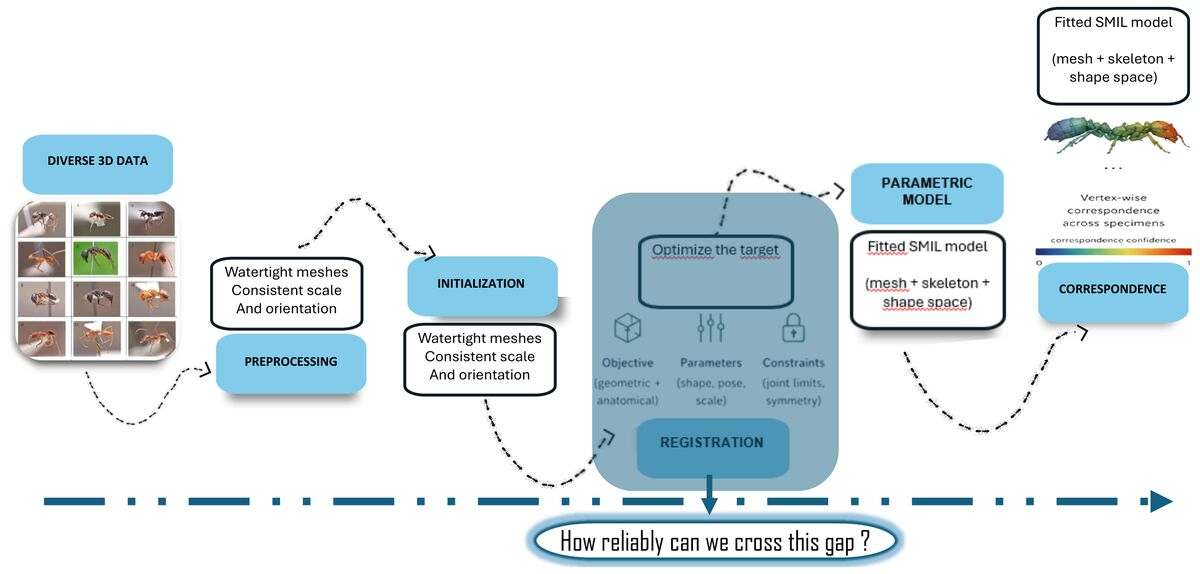
\includegraphics[width=0.9\linewidth]{figures/fig_pipeline_full.jpg}
\caption[The registration pipeline]{The registration pipeline, from diverse raw scans to a
fitted parametric model with vertex-wise correspondence. The correspondence stage did not
exist before this work.}
\label{fig:pipeline}
\end{figure}

\begin{table}[!htb]
\centering
\caption{Stages of the registration recipe.}
\label{tab:stages}
\begin{tabular}{@{}L{0.14\linewidth}L{0.25\linewidth}L{0.27\linewidth}L{0.25\linewidth}@{}}
\toprule
\textbf{Stage} & \textbf{Moves} & \textbf{Observes} & \textbf{Purpose}\\
\midrule
Body & Body chain; legs frozen & Global Chamfer & Place body and coxae\\
Legs & Leg chains; body frozen & Own-territory points per leg &
 Remove six-leg multimodality\\
Joints & All joints; partition kept & Partitioned Chamfer & Refine without
 cross-leg matching\\
Surface, coarse & Pose, shape, scales, $\mathbf d$ ($w_{\mathrm o}=5$) &
 Symmetric Chamfer, 6000 samples & Fit surface; deformation expensive\\
Surface, fine & Same, smaller steps ($w_{\mathrm o}=2$) & Chamfer weight halved,
 regularisers relaxed & Absorb residual detail\\
\bottomrule
\end{tabular}
\end{table}

\subsection{Synthetic correspondence benchmark}
\label{sec:synthetic}

The quantity of interest is not directly observed in an ordinary scan, so every claim
rests on one of two kinds of ground truth. The model can generate its own
targets: sample $(\bm\beta,\bm\theta)$, pose the template, export an anonymous
mesh (optionally degraded), refit it with the production fitter, and compare
fitted vertex $i$ with true vertex $i$. This gives exact correspondence error at
no annotation cost and permits one factor at a time to be varied. Because the
target comes from the model, the benchmark isolates the inverse problem from data
quality and gives a lower bound for real scans; correctness on real specimens is
established by the expert benchmark. The correspondence accuracy is
$A=\frac1{|V|}\sum_i\mathbb 1\big[\arg\min_k\|\hat v_i-v^\ast_k\|=i\big]$,
reported overall and per anatomical part (leg and segment accuracy). It is read
against its own ceiling: feeding the ground-truth mesh itself through the audit
scores below $1$ (about $0.99$ for legs and $0.97$ for segments) because points
near a segment boundary are ambiguous even under exact correspondence, so a gap
is measured to the ceiling and not to unity.

\subsection{Expert Joint Alignment Benchmark}
\label{sec:jab}

For real specimens, an expert placed 3D joints manually, and the Joint Alignment
Benchmark (JAB) was built on them: 11 specimens, 12 strategies, 3 optimiser seeds
and $396$ fits, pre-registered and frozen with a SHA-256 hash before any strategy
was run. Each strategy changes exactly one factor of the production recipe. The
joint error is $e_{sj}=\|\hat j_{sj}-j^\ast_{sj}\|/\mathrm{WL}_s$ in units of
Weber's length (WL, a posture-independent body-size measure), summarised per
specimen by the median over joints and averaged over seeds, with no post-hoc
alignment: Procrustes alignment spreads a few grossly misplaced joints over all
landmarks and masks global placement error~\cite{vonCramon}, and here it
increased the error on 9 of 11 specimens.

Because the reference annotation is itself part of the measurement system, its
coordinate convention was audited before any inference was made from it. Earlier
joint errors had been measured in a frame fitted \emph{to the production
skeleton}; a residual computed on the points used to define an alignment is a
fiducial-type error and says little about error elsewhere~\cite{fitzpatrick}.
Re-registering the annotations through each scan mesh (to a residual below
$10^{-7}$ of the diagonal) moved the measured production error from $42.7\%$ to
$25.1\%$ of WL without touching the fitter. The audit also corrected four
mirror-image annotation scenes, excluded one specimen annotated on another
specimen's mesh, and applied the axis map $(x,y,z)\mapsto(x,z,-y)$ to
surface-landmark coordinates stored in Blender's frame, so that analyses built on
the earlier surface landmarks were retired.

\subsection{Multi-level evaluation protocol}
\label{sec:protocol}

The central methodological challenge is that anatomical correspondence is not
directly observable. Three evidence levels are therefore always used together
(Table~\ref{tab:levels}), and an intervention is adopted only if it does not
degrade levels 1--2 and is checked at level 3 wherever ground truth exists.

\begin{table}[!htb]
\centering
\caption{The three evidence levels of the evaluation protocol.}
\label{tab:levels}
\begin{tabular}{@{}L{0.22\linewidth}L{0.40\linewidth}L{0.30\linewidth}@{}}
\toprule
\textbf{Level} & \textbf{Metrics} & \textbf{Question answered}\\
\midrule
1. Geometric agreement & Chamfer, F-score, per-part variants & Does the fitted
 surface cover the scan?\\
2. Structural integrity & Edge-length distortion, Laplacian and ARAP deviation,
 normal consistency & Was that agreement obtained by distorting the model?\\
3. Anatomical correctness & Synthetic vertex-identity error; expert joint
 error & Does model location $i$ correspond to the anatomical location it
 represents?\\
\bottomrule
\end{tabular}
\end{table}

\textbf{An adversarial test of the metric.} A metric that a targeted attack can
improve by damaging the reconstruction cannot be the sole judge of a fit.
Deliberately snapping distal vertices onto the nearest target surface improves a
per-part surface distance by $53\%$ while edge-length distortion rises $7.5$-fold:
the surface metric improves exactly as the geometric integrity collapses. This is
the clearest justification for the framework.

\textbf{Statistics.} The specimen is the unit of inference. Strategies are
compared with paired Hodges--Lehmann shifts and exact Wilcoxon-inverted intervals,
Holm-corrected across the 11 contrasts, and ranked with a Friedman test~\cite{demsar};
a joint-level mixed model with crossed specimen and joint effects accounts for
the nesting. A strategy is declared \emph{equivalent} to the reference when its
90\% confidence interval lies inside $\pm2.5\%$ of WL, the measured annotation
repeatability, which is the interval-inclusion form of two one-sided tests at
$\alpha=0.05$~\cite{lakens}. At $n=11$ the pre-registered specimen-level test
resolves effects that are consistent across about ten of eleven specimens; smaller
effects are carried by their intervals and by the mixed model.

\section{Algorithmic investigations}
\label{sec:algo}

The investigations follow the inverse problem of Figure~\ref{fig:map}, from the
observation to the search, the constraints and the supervision. Each starts from
the property of the problem that motivates a mechanism, then gives its
formulation and implementation, the experiment that isolates it, and what the
outcome says about the system.

\subsection{Mesh conditioning and skeleton-aware part assignment}
\label{sec:prep}

\textbf{Motivation.} The objective observes only the scan surface, so defects in
that surface are defects in the observation: holes, disconnected fragments,
non-manifold edges and debris, and thin appendages that vanish under naive
simplification (Figure~\ref{fig:raw-scans}). The question is whether repairing the
observation is the lever on registration accuracy (RQ1).

\textbf{Mechanism.} Two repair strategies are complementary. Alpha Wrap~\cite{alphawrap} shrink-wraps the input: a
facet is traversable only if its circumradius exceeds $\alpha$, so cavities and
holes smaller than $\alpha$ stay closed, while the offset sets the distance of the
output from the input; the result is watertight, 2-manifold, intersection-free and
strictly enclosing even for defective input, and a smaller $\alpha$ penetrates
deeper into concavities at the cost of reproducing more of the defects. The
trade-off is therefore set by $\alpha$ relative to the thinnest structure to
preserve, with the offset kept a small fraction of it.
ManifoldPlus~\cite{manifoldplus} instead extracts the exterior faces between
occupied and empty voxels and projects the result back onto the input without
relying on face normals, and can recover zero-volume structures; it serves where
the wrap does not preserve thin parts. Every wrapped mesh passes a fidelity gate on
its worst deviation from the input, and topology-preserving quadric-error
reduction~\cite{qem} completes the stage. On a 50-specimen benchmark every output
was watertight (against none of the inputs) and most were a single connected
component; the fallback was needed on a quarter of the specimens.



\textbf{Evaluation design and finding.} Holding registration fixed, the fit on
cleaned meshes was compared with the fit on raw meshes, and each was scored
\emph{twice}, against the cleaned and against the raw target, so that an easier
scoring target could not be mistaken for a better registration. The sign flips:
cleaning looks like a gain of several per cent against the cleaned target, a loss
against the raw target, and the target-independent metrics show marginally more
distortion after cleaning. Mesh conditioning improves topology and the scoring
target without improving the registration, so input quality is a precondition for
fitting and not the factor that decides anatomical accuracy. The work was
redirected on this basis.

\textbf{Skeleton-aware part assignment.} Several downstream analyses require
deciding which structure a surface point belongs to. Assigning each point to the
nearest coxa anchor starves the middle legs, because a middle-leg point can sit
closer to a neighbouring anchor than to its own. Assigning instead to the nearest
\emph{articulated bone segment}, the standard primitive in skeletal rigging,
treats each leg as the connected chain it is, and raised the macro-averaged F1 of
the part labelling on the template from $0.66$ to $0.83$, with the largest gain at
the middle legs. The model priors of Section~\ref{sec:objective} (joint limits,
bilateral symmetry, the scale barrier) act on the same principle but constrain
\emph{plausibility}: they remove impossible configurations without selecting the
correct one. A Gaussian shape prior added as a stabiliser was removed once it was
found to suppress genuine morphological variation, which is the signal the model
exists to preserve.

\subsection{The Shape Diameter Function as structural information}
\label{sec:sdf}

If identity cannot come from the data term, a pose-independent intrinsic
descriptor might supply coarse anatomical structure before dense correspondence is
resolved. The Shape Diameter Function (SDF)~\cite{sdf}, a scalar measure of local
thickness obtained from rays cast into the solid behind each surface point, is
computable on a raw scan, independent of pose, and small on thin structures. It
separates body from appendage reliably (AUC $\approx0.97$) and is reproducible
across real scans (correlation $0.77$--$0.94$). Instance separation additionally
requires information that distinguishes repeated structures: on real scans the two
mandibles fell into one connected component in $9$ of $12$ specimens, because
connected components cannot split structures that are physically fused and local
thickness does not encode laterality.

This is an instance of a known limitation of intrinsic descriptors: when a shape
has an orientation-reversing self-symmetry, a loss that depends only on intrinsic
quantities has at least two equally valid optima, which is why orientation-aware
formulations were developed~\cite{donati}. The SDF therefore provides class-level
structure (which kind of part) and leaves instance-level identity (which side,
which leg) to be supplied by another source.

\subsection{Learned pose initialisation}
\label{sec:pointnet}

\textbf{Motivation.} The registration objective is non-convex, and its
nearest-surface assignments depend strongly on the initial articulated state. A
fixed canonical pose therefore determines which target regions become the
optimiser's initial attractors, so a poor start commits each leg to the wrong
basin before refinement begins. This motivates an input-conditioned initialiser,
which does not replace optimisation but changes the starting point from which the
non-convex latent space is explored.

\textbf{Formulation and implementation.} The initialiser regresses the initial
rotations of the leg joints from the scan, after which the differentiable fitter
performs local refinement (Figure~\ref{fig:pointnet}). The scan is first
canonicalised using the body-core vertices only, since a frame computed from the
full cloud lets leg pose leak into the reference frame meant to be
pose-invariant. Each of 2048 points carries its canonical coordinates and a
one-hot leg-chain identifier, and the sample is balanced between leg and body
points. A PointNet-style encoder~\cite{pointnet} applies a shared pointwise MLP
and aggregates with max pooling, a symmetric function that makes the descriptor
invariant to point ordering, which a raw scan does not have; a fully connected head
then predicts a continuous 6D rotation representation~\cite{zhou6d} per leg joint,
converted to a rotation matrix by Gram--Schmidt orthogonalisation and trained with
the same geodesic loss used for evaluation, on a 5000-specimen synthetic corpus
generated from the model.

\begin{figure}[!htb]
\centering
\begin{tikzpicture}[every node/.style={font=\footnotesize},
 box/.style={draw,rounded corners=2pt,minimum height=9mm,align=center,fill=white,inner sep=2pt},
 arr/.style={-{Stealth[length=1.6mm]}}]
\node[box] (a) {scan points\\body-core\\canonicalised\\$N\times(3{+}K)$};
\node[box,right=4.5mm of a] (b) {shared\\pointwise\\MLP};
\node[box,right=4.5mm of b] (c) {symmetric\\max-pool};
\node[box,right=4.5mm of c] (d) {global\\descriptor};
\node[box,right=4.5mm of d] (e) {MLP head\\6D rotation\\per leg joint};
\node[box,right=4.5mm of e,fill=blue!10] (f) {$\bm\theta_0$\\differentiable\\fitter};
\foreach \x/\y in {a/b,b/c,c/d,d/e,e/f}{\draw[arr] (\x)--(\y);}
\end{tikzpicture}
\caption[Learned pose initialiser]{Learned pose initialiser. Max pooling makes the
global descriptor invariant to point ordering; the predicted initial leg rotations
seed the differentiable fitter, which performs local refinement.}
\label{fig:pointnet}
\end{figure}

\textbf{Where an initial error does its damage.} Starting from the ground-truth
pose instead of the default repairs the thin distal structures (the pretarsus
error falls about twelvefold) and leaves the proximal attachment unchanged
(Figure~\ref{fig:init-sensitivity}, left). A matched experiment that fixes the total
pose error and varies only its position along the kinematic chain isolates the
reason (right): the same error is recoverable at the tip and damaging at the base,
because a proximal mistake propagates through every joint downstream. At proximal
attachment joints, pose interacts with scale and shape: several latent variables
jointly determine the same surface location, so correct pose alone does not fix it.
The fitter drifts from the pose it is seeded with in every segment, and the error
at the coxa, the clearest instance, correlates with the error in the per-joint
scales and not with pose drift. On exact synthetic meshes the coxa also carries a
label-ambiguity floor from neighbouring coxae, which must be read through.

\begin{figure}[!htb]
\centering
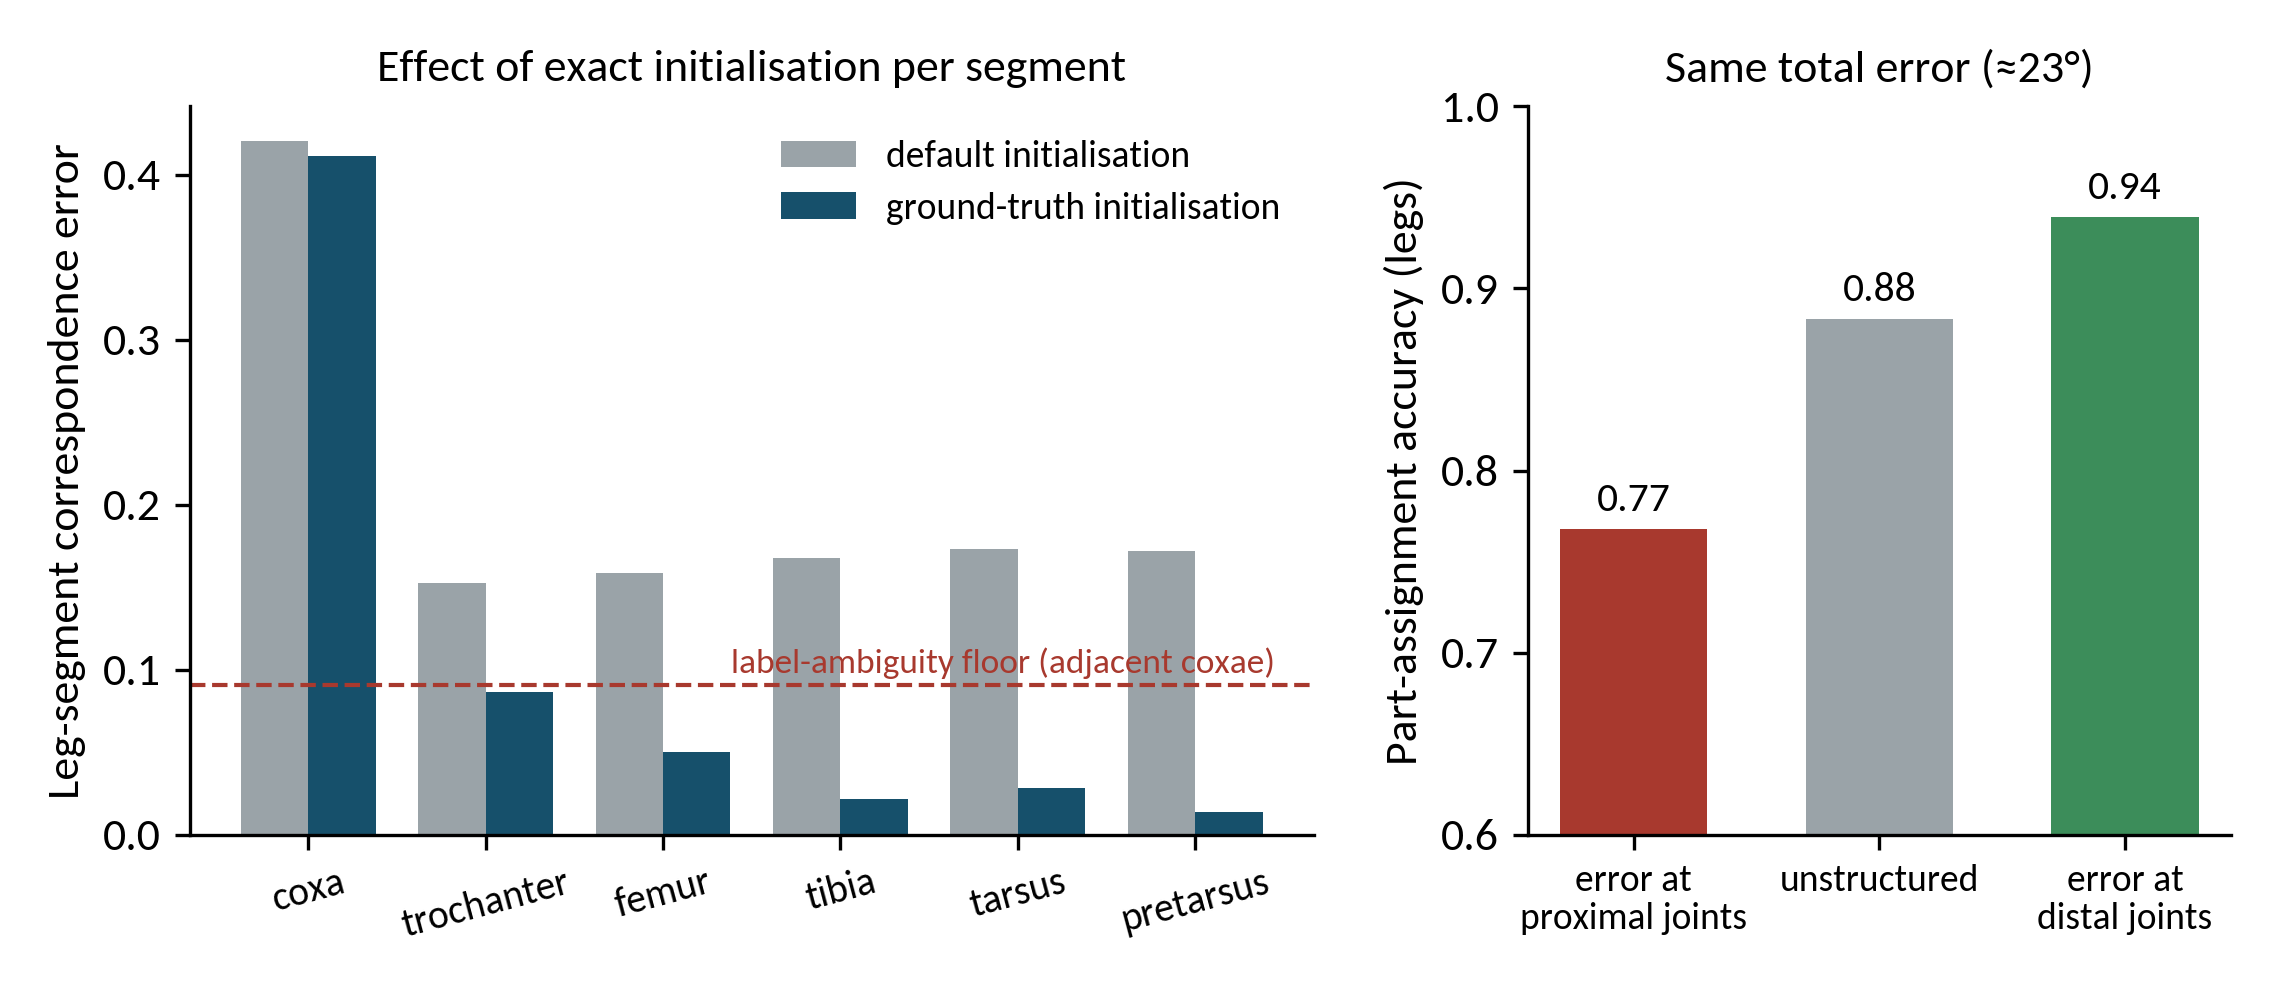
\includegraphics[width=0.74\linewidth]{figures/fig_init_sensitivity.png}
\caption[Sensitivity to initialisation]{Left: per-segment correspondence error under
default and ground-truth initialisation (synthetic, $n=48$); the dashed line is the
label-ambiguity floor at neighbouring coxae. Right: part-assignment accuracy for the
same total pose error ($\approx23^{\circ}$) placed at proximal joints, unstructured, or at
distal joints (synthetic, one seed per condition).}
\label{fig:init-sensitivity}
\end{figure}

\textbf{Transfer.} The learned initialiser improved controlled synthetic recovery
across all metric families. On 50 real specimens, trained at the synthetic
perturbation magnitude, it was significantly worse than the default, and a
controlled sweep of that magnitude moved it monotonically to parity. This separates
the value of input-conditioned initialisation from the question of
synthetic-to-real generalisation: the operative factor is the training
distribution, and the remedy lies there and not in the architecture. The same
sensitivity appears in the expert benchmark, where learned initialisation is
neutral on most specimens and decisive, in the wrong direction, on a few.

\subsection{Sampling and robust optimisation}
\label{sec:sampling}

The surface term is a Monte Carlo estimate,
$\mathcal L_{\mathrm{ch}}\approx\mathbb E_{x\sim p(x)}\big[\operatorname{dist}(x,T)^2\big]$, so the sampling
distribution $p(x)$ determines which anatomical regions contribute most to the
gradient. With $p$ proportional to surface area, the body and head dominate and
thin distal structures are severely under-represented in the optimisation measure.
The template makes this concrete: by dominant skinning weight, one leg has
$200$--$275$ vertices at the coxa and trochanter, $38$ at the tarsus and $8$ at the
pretarsus. Reserving a sampling quota for distal points improved the legs but
starved the antennae and head, which shared the budget; starvation is a real
confound, and controlling it does not by itself create anatomical correspondence.

Robust optimisation addresses points that are simply wrong. Graduated
non-convexity (GNC)~\cite{gnc} starts from a convex surrogate and progressively
hardens a robust cost, needs no initial guess and tolerates large outlier fractions,
without a global-optimality guarantee. Restricted to the leg points it improved
scores under synthetic corruption, whereas applied to the whole body it distorted
the antennae; its effect on clean data was not reproduced under a paired bootstrap,
and the metric behind the early corruption result has since been redefined. GNC is
carried as an additional robustness direction with a defined verification protocol,
not as a component of the shipped recipe.

\subsection{Physical plausibility: inter-part penetration}
\label{sec:penetration}

\textbf{Motivation.} Neither the surface term nor the model priors prevent one part
from passing through another: a leg that crosses the abdomen is a perfectly
reasonable surface to a Chamfer term. Articulated body-model fitting has long
included an interpenetration term for this reason~\cite{bogo}, and a penalty on
inter-part penetration, with an inside/outside decision from nearest-triangle
proximity, was added to the objective.

\textbf{Finding.} On 50 specimens the penalty made contact shallower (mean
penetration depth fell by about $40\%$) without reducing how often collisions
occur (the number of penetrating instances rose by about $17\%$, improving on 23
specimens and worsening on 27), and it degraded surface fit by more than $3\%$ on a
third of specimens. A chain of pre-registered hypotheses localised the mechanism.
That pose is held fixed while the penalty acts was falsified, since the rotations
were in fact used; a clamp on the loss contribution was excluded; and releasing the
smoothness terms that could drag neighbouring vertices into contact gave no
improvement under a causal intervention. Two mechanisms were confirmed: the
asymmetric density of the Chamfer samples across the two parts of a pair, and the
accuracy of the proximity-based inside/outside test, which disagrees with the
generalised winding number~\cite{jacobson} precisely in the direction of the pair
that fails to improve.

\textbf{Implication.} A plausibility constraint is only as reliable as its
inside/outside test and its sampling, and it must be evaluated on both the count and
the depth of violations, since depth alone can improve while the failure persists.
The evidence-supported next step is a winding-number-based test as the loss's core
signal, which was not part of the investigation.

\subsection{Learned dense correspondence}
\label{sec:learned-correspondence}

\textbf{Motivation and formal distinction.} A learned descriptor $f$ supports
\emph{retrieval}, $j^\ast(i)=\arg\min_j\|f(q_i)-f(t_j)\|$, a relation that places no
constraint on coverage or consistency. A dense \emph{correspondence}
$\pi:\mathcal S_A\rightarrow\mathcal S_B$ additionally requires global consistency,
coverage and structural coherence, which is why the correspondence literature
treats local descriptors and globally consistent maps separately, from functional
maps~\cite{fmaps} to embedding formulations~\cite{cse,haugaard} and recent
surveys of the field~\cite{survey}. In optimal-transport form, a coupling $P$ with
prescribed marginals,
$\min_{P\in\Pi(\mu,\nu)}\langle P,C\rangle-\varepsilon H(P)$~\cite{ot}, is what
enforces coverage, and unbalanced variants accommodate incomplete scans.

\textbf{Training logic.} The descriptor shares the backbone and warm start of an
existing contextual embedding (a PointNet++-style network trained with an InfoNCE
objective on exact vertex identity), but is trained for the task actually
evaluated. For a pair of specimens $(A,B)$ and a part, the positive for vertex $i$ is
vertex $i$ on $B$, and the negatives are all other vertices \emph{of the same part}
on $B$: the evaluation task is the loss, and the negatives are within-part by
construction. The input is raw posed coordinates, because normalising away a part's
length and radius removes information that carries correspondence signal. All arms
use one fixed sampling density at training and evaluation (4096 vertices), since the
backbone is out of distribution at five times its training density, with disjoint
training and held-out specimens asserted at run time. Candidates are restricted to
the same part, and the baseline is Euclidean nearest-neighbour matching computed on
exactly the same subsets.

\textbf{Finding.} The learned descriptor beats the Euclidean baseline at the coxa,
where raw proximity is least informative, and the gain strengthens with training; the
other segments do not clear the bar (Figure~\ref{fig:local-vs-dense}a). Pairwise
retrieval accuracy at one joint is thus evidence that learning captures information
raw geometry does not. Deployed in the form the fitter consumes (a target array over
all template vertices), the same descriptor is worse on every one of 48 specimens
than template-embedding lookup in the style of continuous surface
embeddings~\cite{cse}, and its votes collapse onto few template vertices
(Figure~\ref{fig:local-vs-dense}b,c). Restricting the baseline to the descriptor's own
candidate set changes the result by only a few per cent, so the gap is not an
artefact of the comparison. The descriptor is a query-to-query matcher with no
template embedding, so identity of the template has to be carried by reference
specimens; a mechanism that couples the votes into one consistent assignment is what
is missing. This is the benchmark-versus-system gap that evaluation work calls
external validity~\cite{liao}.

\begin{figure}[!htb]
\centering
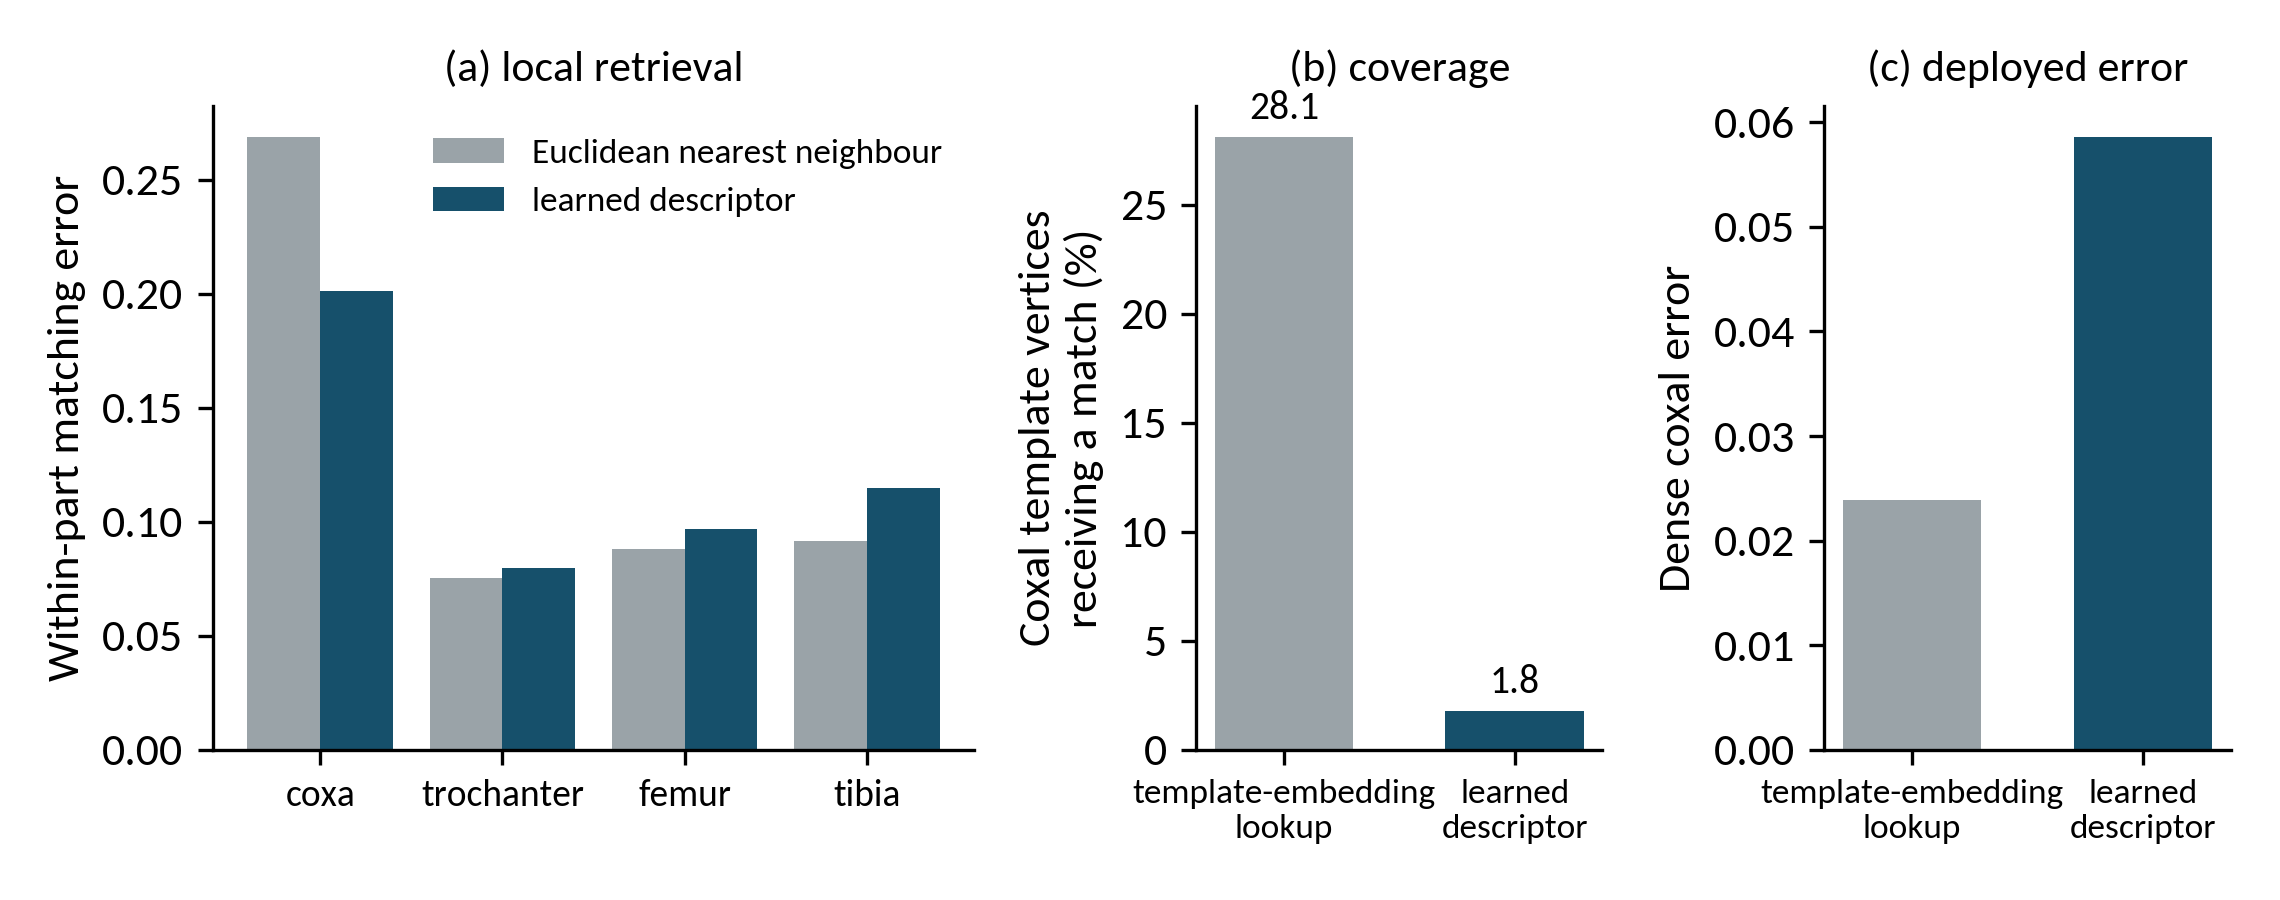
\includegraphics[width=0.70\linewidth]{figures/fig_local_vs_dense.png}
\caption[Local retrieval versus dense assignment]{The same descriptor at two levels.
(a) Within-part matching error against the Euclidean nearest-neighbour baseline: the
learned descriptor wins at the coxa. (b) Fraction of coxal template vertices that
receive a match and (c) dense coxal error when the descriptor is deployed as a full
assignment: strong local retrieval does not imply a usable dense correspondence.}
\label{fig:local-vs-dense}
\end{figure}

A linear probe of the network's features recovers the circumferential angle on tubular
segments far better than chance although retrieval on the same features is poor: the
information is present in the representation and the contrastive objective does not exploit
it, in line with the expectation that correspondence distributions become multi-modal on
symmetric surfaces~\cite{haugaard}. The within-part descriptor above is a query-to-query
matcher with no template embedding, which is exactly what the next subsection adds.

\subsection{A template-embedding head and the location of the residual}
\label{sec:cse}

\textbf{Design.} Every template vertex receives a learned key, and a scan point is matched to the
nearest key~\cite{cse}, so the output is a map over the whole template and not a set of local
votes. The head sits on a hierarchical point-set backbone~\cite{pointnet2} and emits a unit-norm
query per point, trained with a contrastive query--key (InfoNCE) loss on exact vertex identity,
the form that keeps symmetric regions from collapsing to an average~\cite{haugaard}; retrieval is
then a nearest-neighbour search in the embedding, which tolerates noise and partial scans~\cite{coe}.
No hand-designed coordinate system is involved. Each step was gated by a bar fixed before the run.

\textbf{What it established.} A frozen backbone already carried cross-specimen identity, strongly
along a limb and weakly around it, the failure expected of a deterministic embedding on a tubular
part; the contrastive key table improved the
circumferential component by a factor of two to four, the outcome predicted before the head was
written. Two design decisions proved decisive. \emph{How predictions reach the fitter:} given
as direct vertex identity they exceeded exact labels passed through a centroid and
inverse-kinematics conversion, which discards a large share of the achievable gain, so the
mechanism of consumption matters as much as accuracy. \emph{Which predictions to trust without
ground truth:} embedding similarity is entangled with ambiguity, as a point in a confusable
region scores high because it is confusable (the same pathology seen in learned feature
matching~\cite{lightglue}), whereas a cycle-consistency test (scan
point to vertex and back) is structural and, unlike similarity, lowers retrieval error when
used as a filter; it needs no ground truth and no segment whitelist. Deployed this way, the
term improved both part-level and leg-level accuracy on an independent synthetic corpus, and the
fit on nearly every real specimen. Retrieval quality and fitter sensitivity are only loosely coupled, so each gain was tested at the
fitter, and a small-sample estimate was corrected by an independent replication.

\textbf{Where the remaining error lives.} Stratified against a paired ceiling (the ground-truth
mesh scored as the fit), the residual is proximal: the coxa and trochanter own most of it and
the distal segments, which absorbed most of the investigation, own very little. The coxa is not a
correspondence problem: it is fitted as accurately as the body, and its apparent failure comes from
the fitter's general precision coinciding with the spacing between adjacent coxae, which makes a
nearest-vertex metric maximally sensitive there; reweighting the dense term by inverse tolerance
leaves it unchanged. The only intervention that moved it removed free deformation and paid for it in
shape accuracy: the pose--deformation trade-off of Section~\ref{sec:identifiability},
observed at one joint.

\textbf{Hypotheses ruled out.} Table~\ref{tab:closed} lists plausible and costly directions that
were tested against pre-registered bars and rejected; they are as informative as the positive
results.

\begin{table}[!htb]
\centering
\caption{Hypotheses tested against pre-registered bars and rejected.}
\label{tab:closed}
\small
\begin{tabular}{@{}L{0.37\linewidth}L{0.55\linewidth}@{}}
\toprule
\textbf{Hypothesis} & \textbf{Outcome}\\
\midrule
Circumferential signal is absent, so an equivariant network is needed & Present in the features and
 the geometry; the deficit is in the objective\\
Harder same-segment negatives surface it & Overall retrieval improved, the targeted component did not\\
Selecting among several candidates reaches the oracle headroom & Learned ranking and
 optimal-transport assignment~\cite{ot} each captured a small fraction\\
Softer targets or more embedding capacity help & Neither; the keys are not capacity-limited\\
The coxal error is a pose error, a single registration term, or a weighting problem & None of
 these; seeding, ablations and tolerance weighting leave it unchanged\\
\bottomrule
\end{tabular}
\end{table}

\subsection{Objective identifiability, deformation and staged optimisation}
\label{sec:identifiability}

The pose--deformation ambiguity of Section~\ref{sec:objective} predicts a specific
failure: free deformation is an escape hatch. A wrongly posed joint can be repaired
either by rotating it to the right angle or by bending the mesh around the wrong
angle until the surface term is satisfied; the two solutions are nearly
indistinguishable by Chamfer and anatomically unrelated, and only the first preserves
the correspondence needed for measurement (Figure~\ref{fig:gauge}). Neither an unbounded nor a frozen deformation budget is correct, so the
deformation cost acts as a regulariser whose weight sets the conditioning of the
pose; in the earlier synthetic round-trip study, raising that weight was the single most
effective change for correspondence accuracy.

Optimisation dynamics can silently remove part of the latent space. In the
hierarchical schedule the ratio of the pose and shape learning rates left the shape
vector almost fixed (its spread across specimens two to three orders of magnitude
smaller than in the unconstrained schedule), an effect invisible to every surface
metric and found only through a latent-space diagnostic. A second instance came from
the fitting schedule: pose was held fixed for $2000$ of the $2400$ refinement
iterations, so a pose error could only be absorbed by denting the mesh, and the
Chamfer curve descended smoothly regardless; a widened pose-adjustable window
improved nearly every integrity metric at no cost and was adopted.

A third instance concerns priors that carry no anatomical content. The per-joint scale
barrier introduced to curb scale outliers in the head, mandible and antenna groups
reduced its own target statistic, the outlier tail of the scale ratios, by more than
half, yet a test of the mechanism it was meant to correct found no movement, and a
content-bearing replacement tied to a published head-width allometry behaves the same
in the expert benchmark. A prior that fixes a statistic need not fix the anatomy, which
is the distinction between a proxy metric and the construct it stands for: for each
intervention, did it change its intended proxy, and did the anatomical mechanism the
proxy stands for improve?

\subsection{Oracle analysis: what remains when information is supplied}
\label{sec:oracle}

Instead of asking only whether an intervention improves the result, an oracle
ablation supplies the correct answer to one latent sub-problem and measures what
error remains: give the system perfect information about \emph{one} factor, re-run,
and let the residual localise what is unresolved. Each oracle is a minimal change to
Equation~\eqref{eq:objective}: oracle part labels replace the global Chamfer term by one
computed within ground-truth region labels; oracle dense correspondence adds
$w_{\mathrm d}\sum_{y\in Y}\|y-v_{\pi^\ast(y)}\|^2$, matching each target point to the
fitted mesh's own vertex at its true index $\pi^\ast(y)$; and oracle joint positions add
$\lambda\sum_j\|J_j(\bm\beta,\bm\theta,s)-J^\ast_j\|$ with $\lambda=0.03$. They form a
ladder of strictly increasing information, from the identity of a region to the identity
of a vertex to the position of a joint.

\begin{figure}[!htb]
\centering
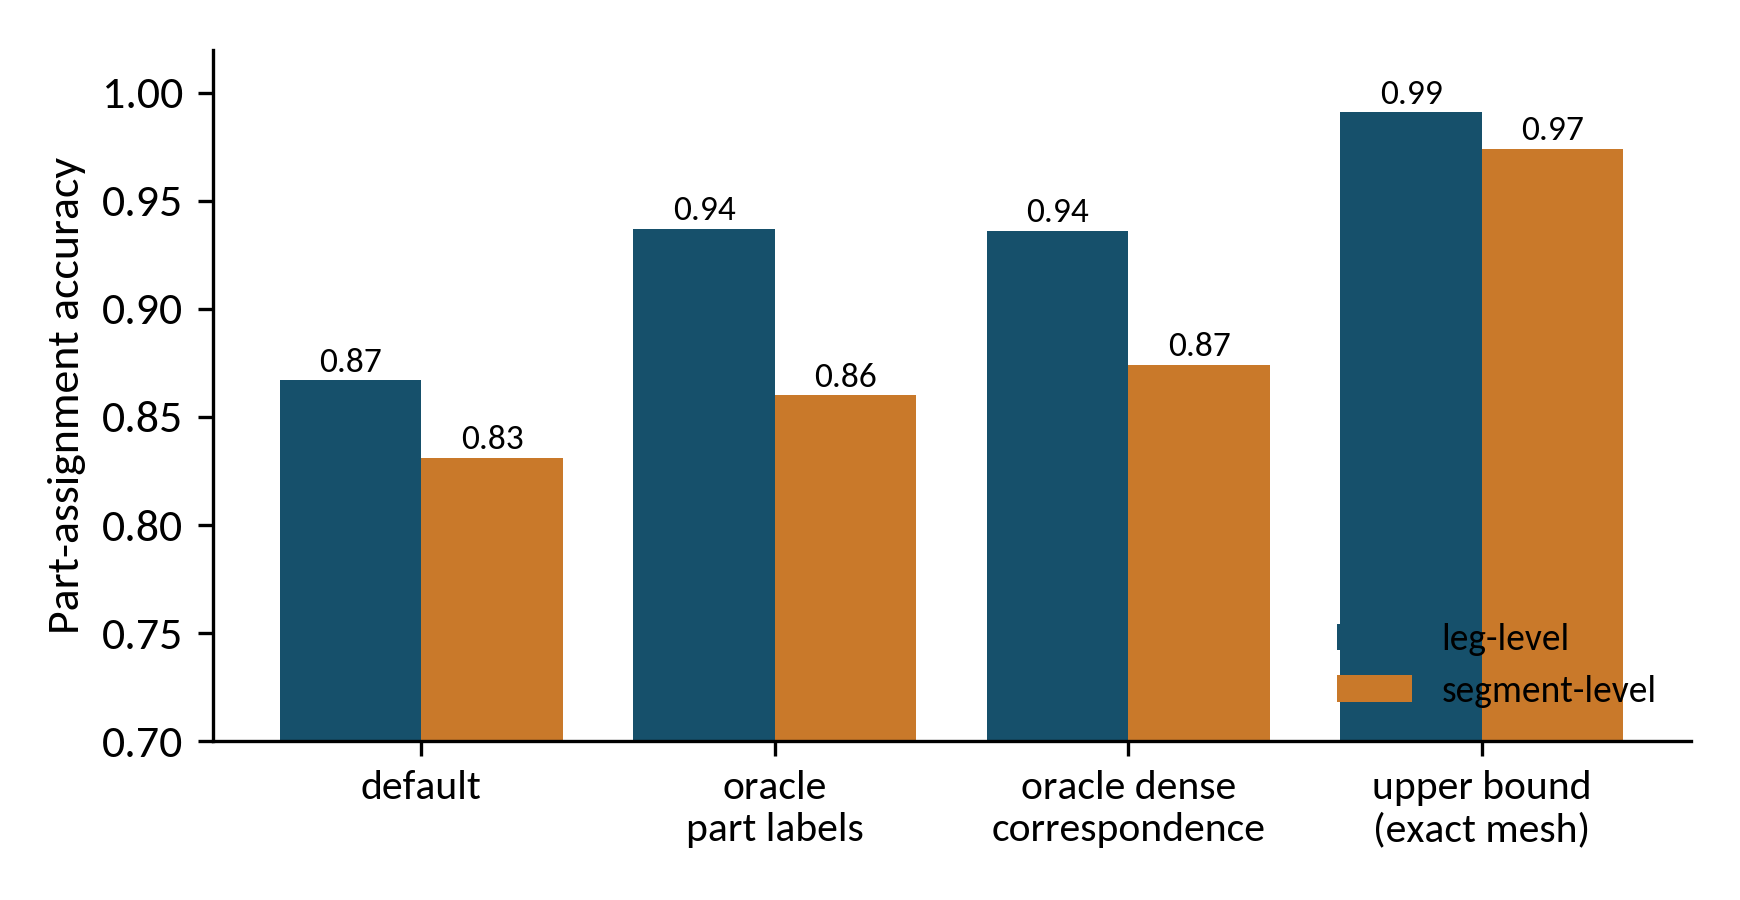
\includegraphics[width=0.46\linewidth]{figures/fig_oracle_ladder.png}
\caption[Oracle ablations]{Part-assignment accuracy on the synthetic benchmark
($n=12$) under oracle part labels and oracle dense correspondence, against the upper
bound of the metric on an exact mesh. Joint-level oracles are evaluated on real
specimens in Section~\ref{sec:skeleton}.}
\label{fig:oracle}
\end{figure}

Supplying the true region of every target point raises accuracy only partially, and
most of the gain comes from a minority of specimens. Supplying exact per-vertex
correspondence improves within-part accuracy on every specimen yet remains clearly
below the upper bound (Figure~\ref{fig:oracle}). Regional identity and within-region
localisation are therefore distinct problems, and correspondence is not the only
missing ingredient: the objective, the optimisation trajectory and the deformation
freedom keep limiting the fit even when correspondence is solved. The oracle that
supplies joint positions is the only one on real data, and it leads into the next
section.

\section{Anatomical recovery and measurement validity}
\label{sec:validity}

Sections~\ref{sec:framework} and~\ref{sec:algo} established what the objective
observes and what each mechanism adds. This section asks what the recovered
representation supports as a measurement, using the vocabulary that the experiments
force. \emph{Geometric agreement}: the surfaces overlap. \emph{Surface
correspondence}: points are mapped geometrically. \emph{Anatomical correspondence}:
the mapping preserves anatomical identity. \emph{Parametric recovery}: the recovered
$\bm\beta,\bm\theta$ have a stable meaning across specimens. \emph{Measurement
validity}: a quantity extracted from those parameters agrees with a reference. Each
level is necessary for the next and none implies it.

\subsection{Surface agreement versus anatomical correctness}
\label{sec:geometric-agreement}

\textbf{Question and test.} If a fit scores better on the objective's own terms, is
its skeleton better? Within the Joint Alignment Benchmark, the free-form deformation
and normal regularisation were removed from the production recipe, and surface and
skeleton were compared across twelve strategies. \textbf{Finding.} This produced the
\emph{closest} surface of all twelve strategies (about $0.45\times$ the Chamfer
distance) and one of the worst skeletons (joint-level ratio $1.25$, worse on 8 of 11
specimens), and no strategy lay in the quadrant of better surface \emph{and} better
skeleton (Figure~\ref{fig:dissociation}). Removing the regularisation inflated the
free-form deformation roughly nine-fold: the surface was fitted by moving the skin
and not the skeleton, which is the prediction of Equation~\eqref{eq:gauge}. The
joint-level model resolves the effect, and the specimen-level test, whose threshold
is about ten of eleven consistent specimens, shows the same direction on eight.

\textbf{Implication.} Surface agreement can certify coverage of the scan and nothing
about anatomical identity, so a surface metric must not be used to choose a method
for anatomical accuracy. The dissociation of fit error from target error is
established in registration more generally~\cite{fitzpatrick}; what the benchmark
adds is its measured size in a deformable articulated model, under a pre-registered
single-factor ablation, together with the adversarial demonstration of
Section~\ref{sec:protocol}.

\begin{figure}[!htb]
\centering
\begin{minipage}[b]{0.46\linewidth}
\centering
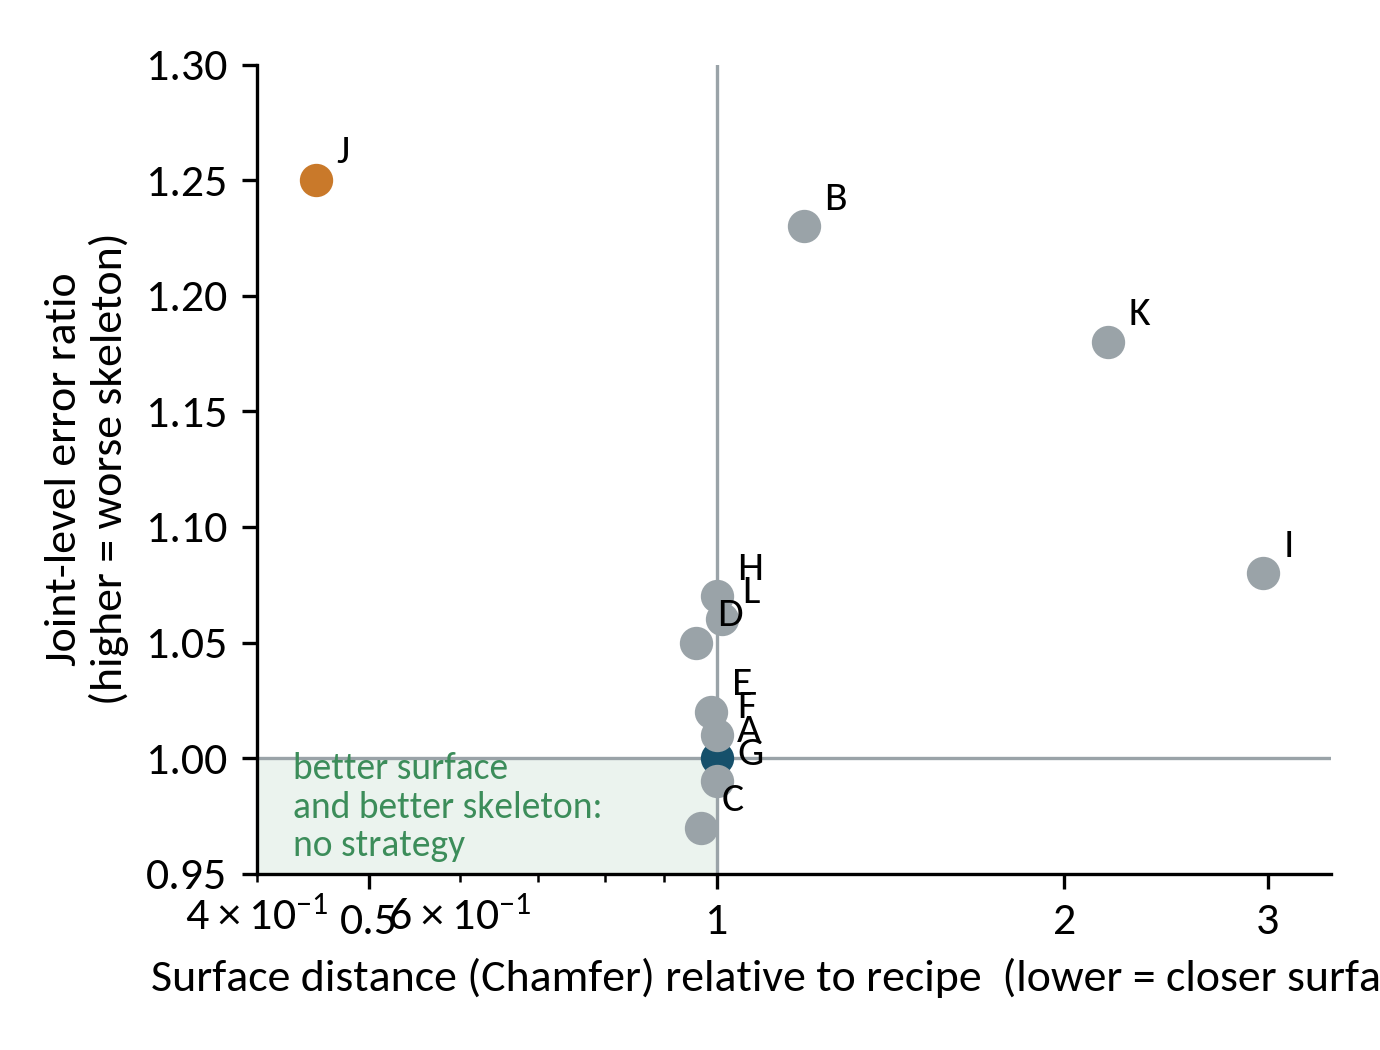
\includegraphics[width=\linewidth]{figures/fig_dissociation.png}
\end{minipage}\hfill
\begin{minipage}[b]{0.48\linewidth}
\centering
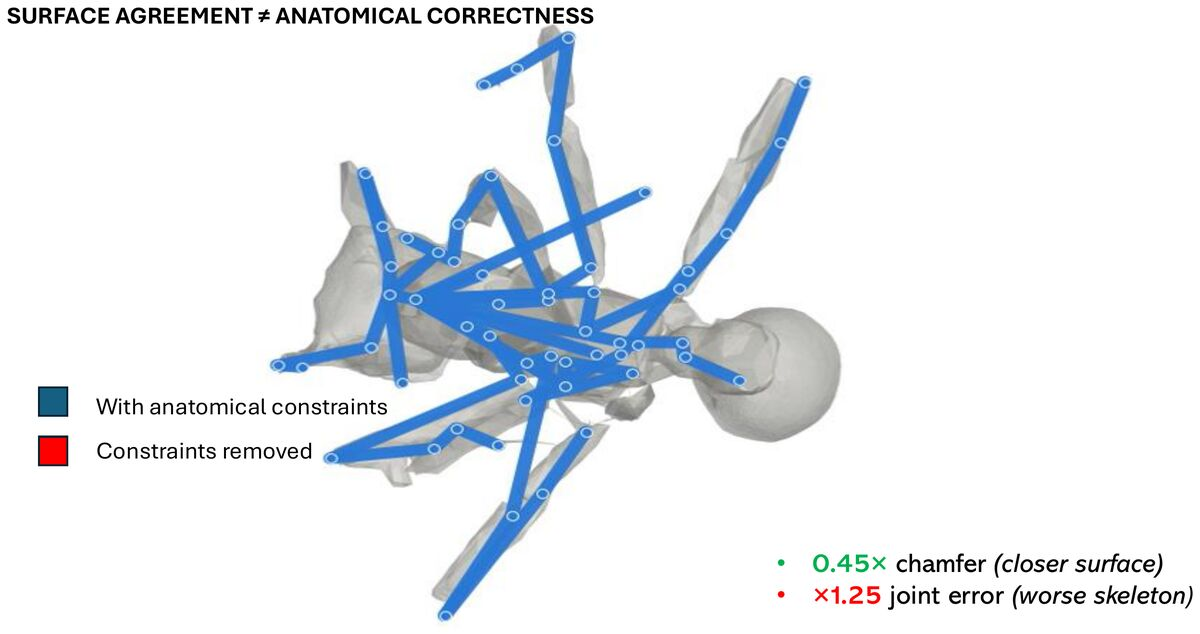
\includegraphics[width=\linewidth]{figures/fig_geometric_agreement.jpg}
\end{minipage}
\caption[Surface agreement and anatomical correctness]{Left: surface distance against
skeleton error across the twelve strategies (letters as in Figure~\ref{fig:jab}); the
strategy with the closest surface, J, has one of the worst skeletons, and none improves
both. Right: the skeleton overlay with the regularisation active; removing it yields a
closer surface and a worse skeleton.}
\label{fig:dissociation}
\end{figure}

\subsection{Skeleton recovery against the expert reference}
\label{sec:skeleton}

\textbf{What the objective observes, and what the output requires.} The objective
observes surface geometry, normals, mesh regularity, symmetry and rotation ranges.
The desired output additionally requires joint location, anatomical identity and
within-structure correspondence. No term of the objective explicitly observes joint
position, and reweighting an existing term cannot recover information that the
objective does not observe. The benchmark tests this directly.

\textbf{Evidence.} Production joint error is about a quarter of Weber's length (median
$25.1\%$, 95\% CI $17.5$--$44.8$). Supplying expert joint targets during fitting lowers
the error to $17.4\%$, from $26.9\%$ in a paired control that re-fits the same specimens
without targets ($10$ of $11$ improve; the control itself leaves the error unchanged), so a
better skeleton exists within the model's own shape budget. Yet no single-factor change
to the recipe improves joint alignment reliably, and the recipe ranks best of the
twelve (Figure~\ref{fig:jab}, left). Supervision supplied for every region
\emph{except} one leaves that region essentially unchanged, with every held-out
interval including zero: supervision acts locally and does not propagate. Alignment is
largely won in a single place, the part-wise leg stage, which improved all eleven
specimens, while later steps add little (Figure~\ref{fig:jab}, right); the scale
regularisation and the allometric prior are joint-neutral.

\begin{figure}[!htb]
\centering
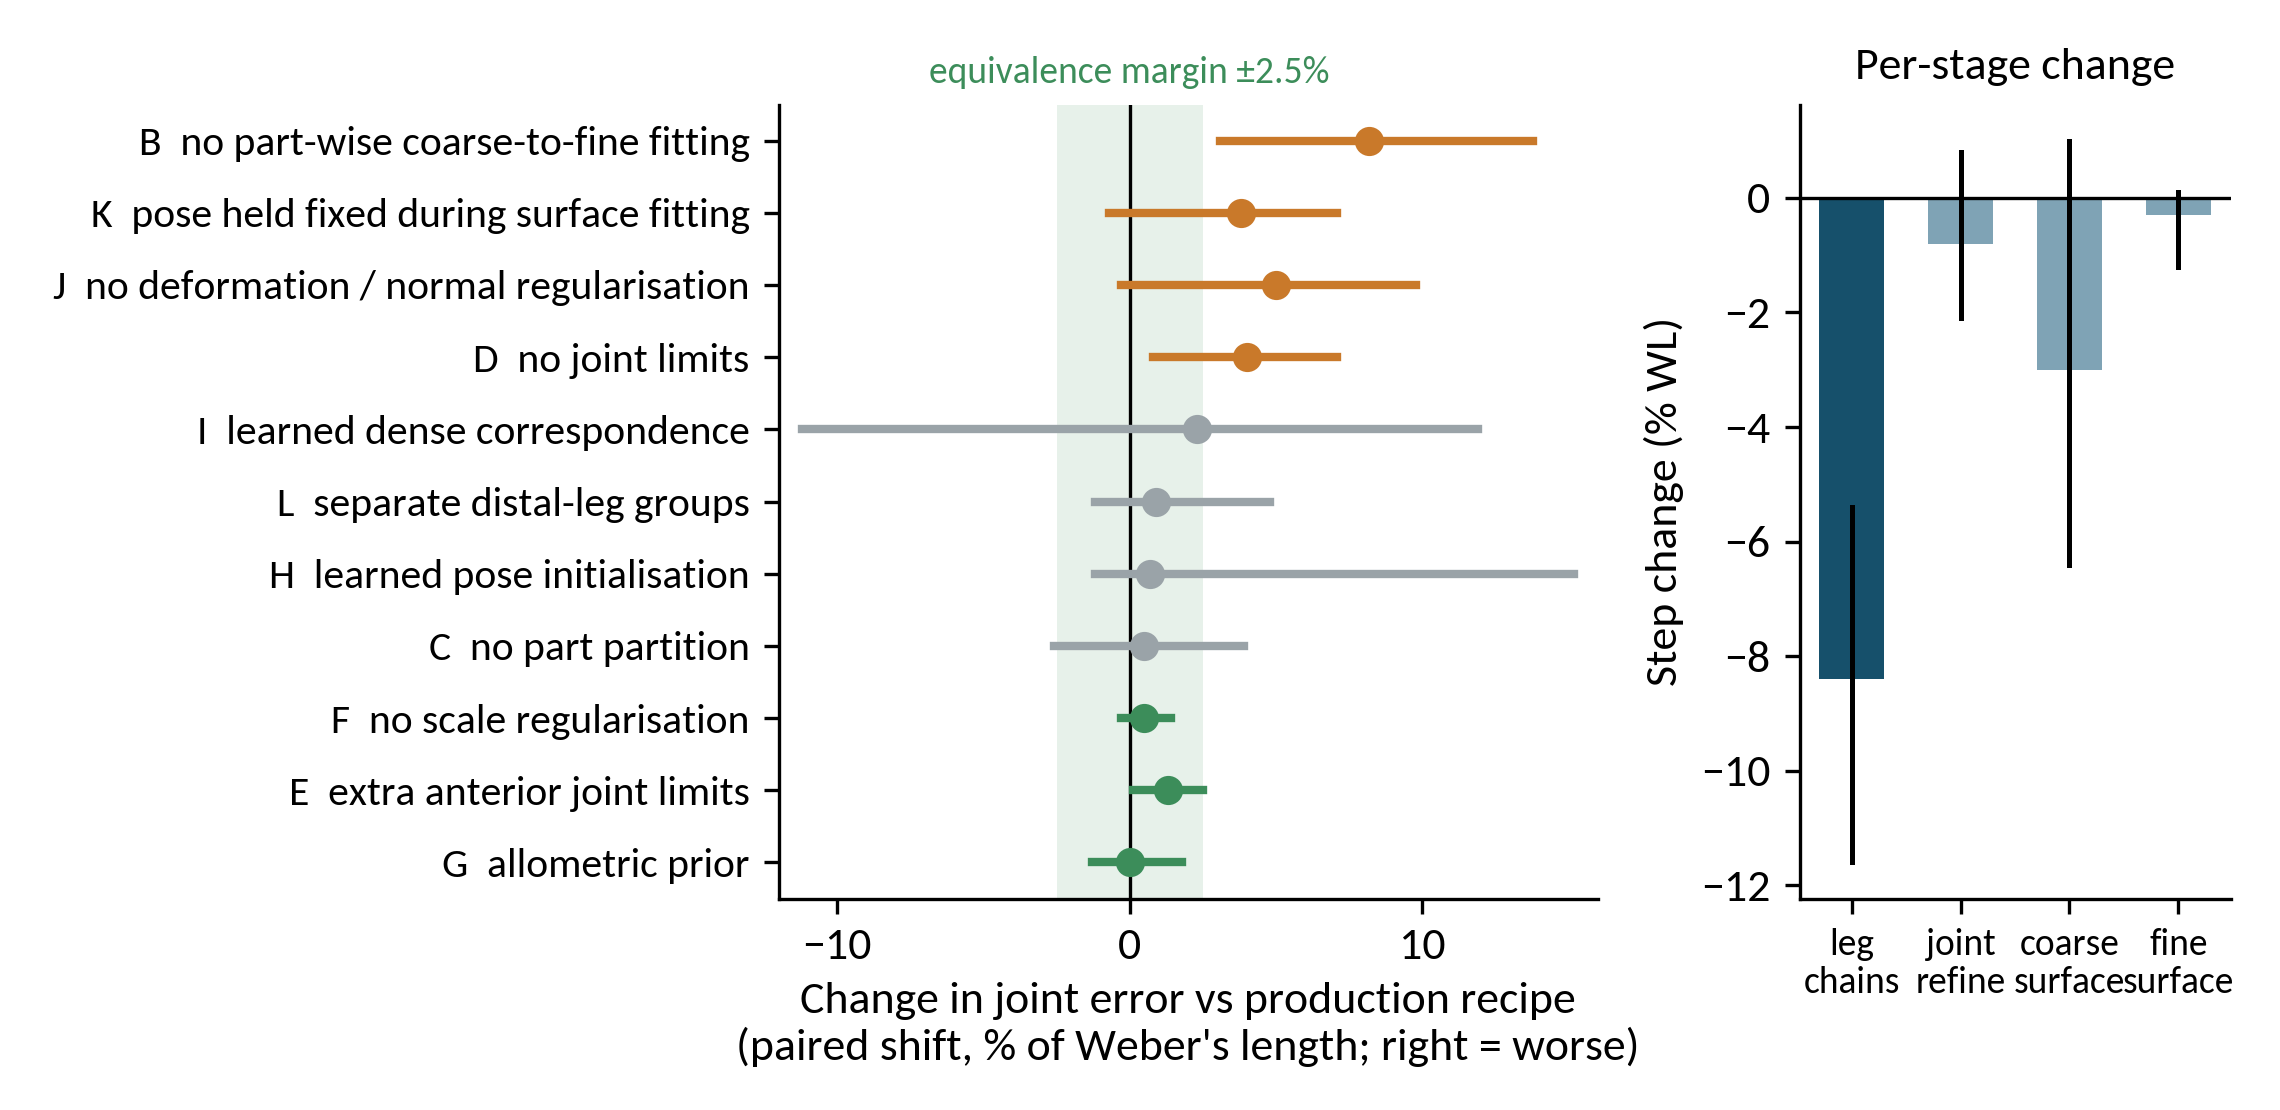
\includegraphics[width=0.78\linewidth]{figures/fig_jab_contrasts.png}
\caption[Joint Alignment Benchmark]{Joint Alignment Benchmark ($n=11$ specimens, 396
fits). Left: paired change in joint error for each single-factor strategy against the
production recipe, with 95\% intervals; the shaded band is the $\pm2.5\%$ equivalence
margin, and green marks strategies equivalent to the recipe. Right: per-stage change in
joint error within the recipe.}
\label{fig:jab}
\end{figure}

\textbf{Structure of the error.} The error is not uniform
(Figure~\ref{fig:structured-error}): proximal leg joints are placed at about
$12$--$13\%$ of WL, the body axis at $24\%$, and the mandibles, antennae and thin
distal segments at $43$--$56\%$. A variance decomposition attributes far more of the
spread to \emph{which joint} and \emph{which specimen} than to the optimiser seed, so
the failure is anatomically structured. The ordering is the expected one, since pose
estimation has long reported error growing along a kinematic chain; what the benchmark
supplies is the usable per-region number.

\begin{figure}[!htb]
\centering
\begin{tikzpicture}
\begin{axis}[ybar,width=0.60\linewidth,height=4.2cm,bar width=7pt,ymin=0,ymax=68,
 symbolic x coords={Coxae,Troch./femur,Body axis,Mandibles,Antennae,Tibia/tarsus},
 xtick=data,x tick label style={rotate=25,anchor=east,font=\footnotesize},
 ylabel={error (\% WL)},ylabel style={font=\footnotesize},tick label style={font=\footnotesize},
 nodes near coords,every node near coord/.append style={font=\footnotesize}]
\addplot[fill=blue!55] coordinates {(Coxae,11.6)(Troch./femur,12.9)(Body axis,24.1)(Mandibles,42.8)(Antennae,54.9)(Tibia/tarsus,56.3)};
\end{axis}
\end{tikzpicture}
\hfill
\begin{tikzpicture}
\begin{axis}[ybar,width=0.30\linewidth,height=4.2cm,bar width=9pt,ymin=0,ymax=0.5,
 enlarge x limits=0.3,
 symbolic x coords={Joint,Specimen,Seed},xtick=data,tick label style={font=\footnotesize},
 x tick label style={rotate=25,anchor=east},
 ylabel={log-scale variance},ylabel style={font=\footnotesize},nodes near coords,
 every node near coord/.append style={font=\footnotesize,/pgf/number format/fixed,/pgf/number format/precision=2}]
\addplot[fill=orange!70] coordinates {(Joint,0.36)(Specimen,0.17)(Seed,0.02)};
\end{axis}
\end{tikzpicture}
\caption[Structure of the skeleton error]{Left: median skeleton error by region for the
production recipe. Right: variance decomposition across the same fits; the optimiser seed
contributes almost nothing.}
\label{fig:structured-error}
\end{figure}

\subsection{From recovered parameters to measurable traits}
\label{sec:measurement}

A number extracted from an articulated fitted model is not automatically a
morphometric. Four validity axes fail independently, which is why one is not enough: the
trait's endpoints sit on the structure it is named after (\emph{anatomical}); it is stable
when only the articulation changes (\emph{pose invariance}); it reproduces a known scaling
relationship (\emph{biological}); and it is internally consistent, for instance in its
bilateral asymmetry, since near-symmetric animals make left--right disagreement a
measure of error (\emph{consistency}). A trait can be perfectly pose-stable and still be
anatomically wrong, measuring the wrong structure consistently, so any single axis can
certify a fit that is wrong. The internal-consistency axis ranks traits correctly but is a
trait-level screen and not a per-specimen confidence score, because within a trait
asymmetry does not predict pose contamination.

Manual joint annotation by an expert (Figure~\ref{fig:ground-truth}) provides the reference
for the skeleton-based axes. Head width, read from two reporter bones placed on the head
capsule, is the trait that carries this validation. It is the most pose-invariant trait examined (its value changes by
about $0.1\%$ when only articulation changes), its endpoints are defined by a part extent
and not by landmark indices, and it reproduces the allometric scaling of head width against
body length (exponent $1.21$, interval $1.15$--$1.26$, against $1.24$ in the reference
data). Against the reference head widths supplied with the \emph{Atta vollenweideri} data
set for 20 workers, the mean absolute difference is about $4\%$
(Figure~\ref{fig:head-width}). Agreement in millimetres is partly shared with the
reference because scale is restored from body length, so the dimensionless ratio of head
width to body length is the informative test; it also agrees (concordance coefficient
$0.86$; the mean relative difference is the same as for the absolute value by
construction, since body length cancels, so the informative change is the fall in
concordance once the shared size is removed), with a modest size-dependent bias that is the same effect as the slightly
compressed scaling exponent: the model slightly compresses the allometric relationship at
the extremes of the size range. The two head-width definitions tested are not
interchangeable (the reporter-bone distance is essentially unbiased, whereas a
Type~III extent carries a systematic $+2\%$ bias), so the definition is part of the
measurement.

\begin{figure}[!htb]
\centering
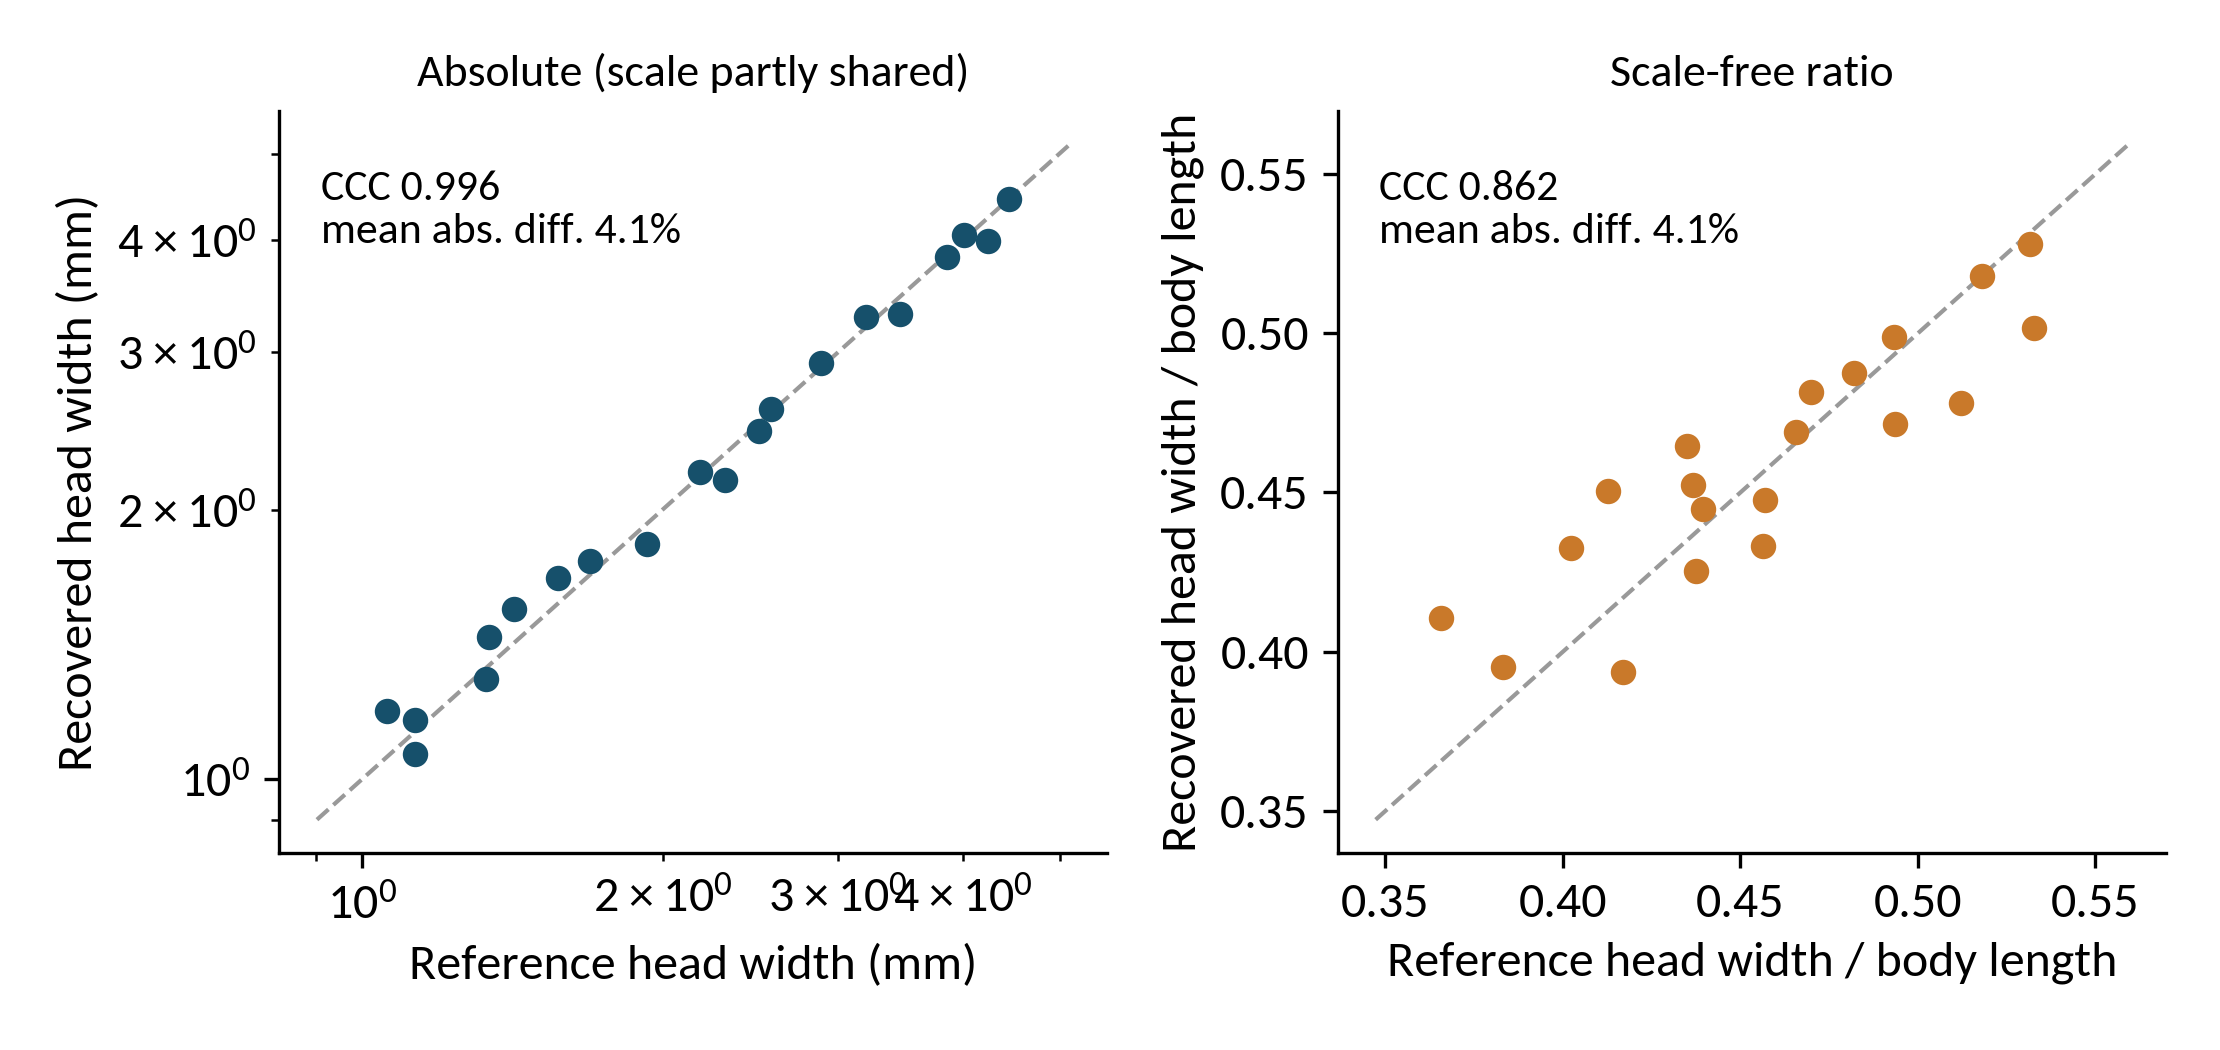
\includegraphics[width=0.62\linewidth]{figures/fig_head_width_agreement.png}
\caption[Head-width agreement]{Head width recovered by the registration against the reference
table supplied with the data set (20 \emph{Atta vollenweideri} workers). Left: absolute head
width (log scale; scale is partly shared through body length). Right: scale-free ratio of
head width to body length, the independent test; the mean relative difference is
identical to the left panel by construction (body length cancels), whereas concordance
falls from $0.996$ to $0.86$. Dashed lines are identity.}
\label{fig:head-width}
\end{figure}

The same framework identifies where measurement should not be trusted. Traits whose
endpoints are rig pivots instead of surface-defined points, or that are sensitive to
articulation, require a different definition before use. Registration of an independent
ethanol-preserved worker corpus sits at a measurable noise floor, at which two conspecific
workers are only about $7\%$ closer than unrelated ants, and distal leg and antenna segment
lengths, the structures that the expert benchmark and the sampling analysis identify as the
least constrained, disagree between nest-mates as much as between unrelated ants.
Region-level reliability is therefore taken from the expert benchmark, and genus-level
structure in shape-ratio traits is reported as an exploratory population-level result.

\begin{figure}[!htb]
\centering
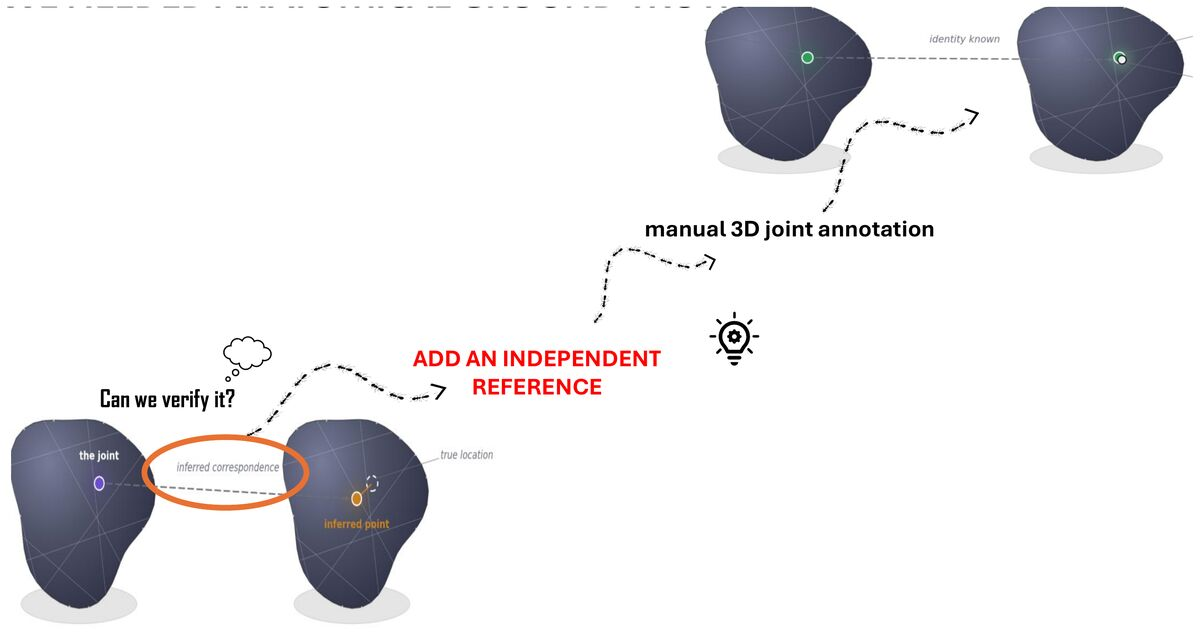
\includegraphics[width=0.34\linewidth]{figures/fig_ground_truth_annotation.jpg}
\caption[Expert joint annotation]{Manual 3D joint annotation as an independent reference,
with identity known by construction, against which the model's inferred correspondence can be
verified and not merely inspected.}
\label{fig:ground-truth}
\end{figure}

\subsection{Scale-dependent validity}
\label{sec:validity-scale}

``The registration is valid'' is therefore not one claim but five, holding at different
scales and supported by different evidence (Table~\ref{tab:validity}). A model can give an
accurate population-level or single-trait measurement while failing to preserve the
individual-level correspondence needed for specimen-by-specimen comparison, and each
statement is supported only at its own level. The expert-supervised fit quantifies the
headroom available; since expert joints are unavailable at inference time, supplying an
equivalent signal automatically is the objective it motivates.

\begin{table}[!htb]
\centering
\caption{Levels of registration validity and the evidence for each.}
\label{tab:validity}
\begin{tabular}{@{}L{0.20\linewidth}L{0.34\linewidth}L{0.34\linewidth}@{}}
\toprule
\textbf{Level} & \textbf{Question} & \textbf{Evidence}\\
\midrule
Geometric agreement & Do the surfaces overlap? & Chamfer, F-score; misleading alone
 (Section~\ref{sec:geometric-agreement})\\
Surface correspondence & Are points mapped geometrically? & Nearest-surface matching;
 label-invariant (Section~\ref{sec:objective})\\
Anatomical correspondence & Does vertex $i$ mark the same structure across specimens? &
 Synthetic oracles, expert benchmark\\
Parametric recovery & Do $\bm\beta,\bm\theta$ mean the same thing across specimens? &
 Region-dependent; nest-mate agreement\\
Measurement validity & Does a derived quantity match a reference? & Head width on 20
 workers; four validity axes\\
\bottomrule
\end{tabular}
\end{table}

\section{Discussion}
\label{sec:discussion}

\subsection{What the experiments establish}

Table~\ref{tab:questions} collects the technical questions, the main finding for each
and the evidence basis. Read together, the experiments indicate that the dominant
difficulty is not surface alignment but recovery of a unique anatomical explanation
from an observation that lacks explicit identity information, and that each
mechanism acts on that ambiguity: free deformation can absorb a pose error, local
learned votes can be accurate and globally inconsistent, and supervision constrains
only where it is supplied.

\begin{table}[!htb]
\centering
\caption{Technical questions, main findings and evidence basis.}
\label{tab:questions}
\begin{tabular}{@{}L{0.30\linewidth}L{0.40\linewidth}L{0.22\linewidth}@{}}
\toprule
\textbf{Technical question} & \textbf{Main finding} & \textbf{Evidence basis}\\
\midrule
Does cleaner input improve registration? & Topology improves; registration does
 not, once scored against both targets & Matched A/B, 50 specimens\\
Can surface agreement certify anatomy? & No; deformation can reduce surface error
 while worsening skeletal alignment & Expert benchmark, controlled ablation\\
Where does correspondence error arise? & Regional identity and within-region
 localisation are distinct & Synthetic round-trip, oracle ablations\\
Does initialisation determine recovery? & Sensitivity depends on position in the
 articulated chain and on the training distribution & Synthetic perturbation study,
 real scans\\
What information does the objective lack? & No term observes joint position; supervision
 acts locally & Expert benchmark, held-out regions\\
Can recovered parameters serve as measurements? & For validated quantities and
 scales, not uniformly & Reference table, noise floor\\
\bottomrule
\end{tabular}
\end{table}

\subsection{Relation to existing work}

\textbf{Parametric articulated models.} SMPL~\cite{smpl} learns a human shape and
pose space under a fixed topology; SMAL~\cite{smal} learns a quadruped shape space
from scans of toy figurines through a part-based registration, and the SMALify
procedure~\cite{smalify} fits it to images and video by energy minimisation.
SMILify~\cite{smilify} generalises this to arbitrary rigged templates and optimises
shape, pose, scale and per-vertex deformation against the target, which introduces
the freedom that Section~\ref{sec:identifiability} analyses.

\textbf{Point-cloud registration and learned matching.} Deep Closest Point~\cite{dcp}
replaces iterative closest point's greedy matching with a learned embedding, an
attention module that approximates combinatorial matching and a differentiable
rigid fit; PREDATOR~\cite{predator} lets two clouds exchange information through
an overlap-attention block to handle low overlap; GeoTransformer~\cite{geotransformer}
encodes pairwise distances and triplet-wise angles and matches coarse superpoints
before dense points. These are rigid problems. The present setting is a model-based
one, in which the match is constrained to the image of an articulated parametric
model, and the initialiser of Section~\ref{sec:pointnet} is closer to a
PointNet-based pose regressor~\cite{pointnet}, whose max-pooling construction is
permutation invariant and robust to missing points.

\textbf{Non-rigid surface correspondence.} Functional maps~\cite{fmaps} represent a
correspondence as a linear map between function spaces in a Laplace--Beltrami basis
and assume near-isometry. Fully intrinsic formulations cannot separate a shape from
its mirror image when orientation-reversing symmetries exist~\cite{donati}, the
limitation that Section~\ref{sec:sdf} meets on ant scans. Embedding formulations
learn dense correspondence from vertex identity~\cite{cse}, and correspondence
distributions become multi-modal on symmetric surfaces without symmetry
supervision~\cite{haugaard}. Implicit-function formulations learn probabilistic
embeddings with a confidence that a correspondence exists on the target for
topology-varying shapes~\cite{liu2020}. A recent survey~\cite{survey}
organises the field by correspondence problem, by paradigm for generating and
refining correspondences, by evaluation strategy and by topology, and notes that
formulations differ with the application and the input data.

\textbf{Robust and structured geometry.} As-rigid-as-possible
modelling~\cite{arap}, graduated non-convexity~\cite{gnc} and defect-tolerant
repair~\cite{alphawrap,manifoldplus} supply the regularisation, robustness and
conditioning ingredients used here.

\textbf{What differs in this setting.} In the articulated parametric setting,
correspondence is coupled to recovery of latent articulated parameters and residual
deformation, the scan is noisy and incomplete, and the quantity to be validated
(anatomical identity) is not available from any scan. The contribution is therefore
the diagnostic framework that separates these couplings, not a new matching
architecture.

\subsection{General technical implications}

The mechanisms generalise beyond ants without being claimed as universal. Any
registration objective built from a symmetric surface distance is label-invariant,
so any model with an additive residual field after skinning has a
pose--deformation equivalence whose conditioning is set by the regulariser. Any
sampling-based surface term weights regions by sampling measure. Any local
descriptor must be evaluated as the assignment the downstream consumer needs, and
any benchmark that scores a proxy can be moved by changing the scoring target.
Whether each failure recurs on other body plans is an empirical question the same
framework is built to answer.

\subsection{Scope of the evidence}

The conclusions are bounded by the data in a precise way. The expert benchmark has
11 specimens, so the pre-registered specimen-level test resolves effects that are
consistent across about ten of eleven specimens, and smaller effects are carried by
intervals and the joint-level model. Synthetic targets come from the model and give
a lower bound for real scans. A fixed topology and a 25-dimensional shape basis define
what the model can express, and residual deformation is ambiguous with pose by
construction. Annotation has its own repeatability, trait definitions are coupled to
scale, and a population-level result does not carry over automatically to individual
specimens. The ground-truth audit retired earlier analyses built on the superseded
reference; every result reported here rests on the corrected benchmark or on exact
synthetic ground truth.

\section{Conclusion and outlook}
\label{sec:conclusion}

\subsection{Technical synthesis}

The starting observation was that an optimiser can succeed while a registration
fails. The investigation traced this to one structural fact: the scan supplies
surface geometry, whereas anatomical correspondence is an intended consequence of
the recovered parameters and is constrained only through the model, its priors and
independent verification. Four distinctions summarise the
outcome: representability is not recoverability; regional identity is not
within-region location; plausibility is not correspondence; and fit quality is not
measurement validity. Each was the concrete reason that a plausible intervention
failed to deliver what it was built for.

Technically, the investigation extended the pipeline across mesh conditioning,
anatomical priors, learned point-cloud initialisation, sampling-aware and robust
optimisation, learned correspondence and hierarchical fitting, while introducing
synthetic and expert-grounded instruments to evaluate these mechanisms
independently. Taken together, the experiments indicate that the dominant
difficulty is not simply surface alignment but recovery of a unique anatomical
explanation from an observation that lacks explicit identity information. A useful
parametric representation is defined not only by what it can represent but by what
anatomical meaning survives its recovery from data: a reconstruction is not yet a
phenotype.

\subsection{Research directions}

Each direction follows from a diagnosed limitation (Table~\ref{tab:roadmap}), and
none was implemented.

\begin{table}[!htb]
\centering
\caption{Diagnosed limitations and the research directions they motivate.}
\label{tab:roadmap}
\begin{tabular}{@{}L{0.40\linewidth}L{0.52\linewidth}@{}}
\toprule
\textbf{Diagnosed limitation} & \textbf{Next technical direction}\\
\midrule
Remaining circumferential ambiguity and the fitter's precision at the proximal joints & Objective
 that exploits the present circumferential signal; functional maps~\cite{fmaps} for global coupling\\
Joint position is not observed & Skeleton-conditioned correspondence, a learned 3D
 joint predictor\\
Free deformation can absorb pose & Structured, diffeomorphic deformation\\
Synthetic learning transfers unevenly & Scan-realistic corruption and domain
 randomisation\\
Part identity does not give precise location & A continuous anatomical canonical
 field with uncertainty, in the spirit of probabilistic implicit
 embeddings~\cite{liu2020}\\
\bottomrule
\end{tabular}
\end{table}

The most ambitious direction is an anatomical canonical field that predicts, for
every observed point, its part, joint-relative coordinates, laterality and a
confidence, so that correspondence becomes the mapping of a scan into a canonical
anatomical coordinate system: exactly the information the diagnosed objective lacks.

\subsection{Broader significance}
\label{sec:significance}

The ant is a useful test case because it forces diversity, articulation, difficult geometry
and correspondence to be handled at once (Figure~\ref{fig:corpus}): genera differ in body
plan and posture, the structures of interest are thin and articulated, and the data are
imperfect. The aim, however, is broader than one good ant model. The longer-term objective
is to use what is learned here to build purpose-built articulated models for the body plans
that a scientific question actually requires, spanning other animals within a single
construction and fitting pipeline and not one predefined model family, as the mouse and
multi-species insect models already built with the same framework~\cite{smilify} begin to
show. It extends equally to human-centred applications, where generic parametric models can
impose restrictions that are inappropriate to the question being asked.

\begin{figure}[H]
\centering
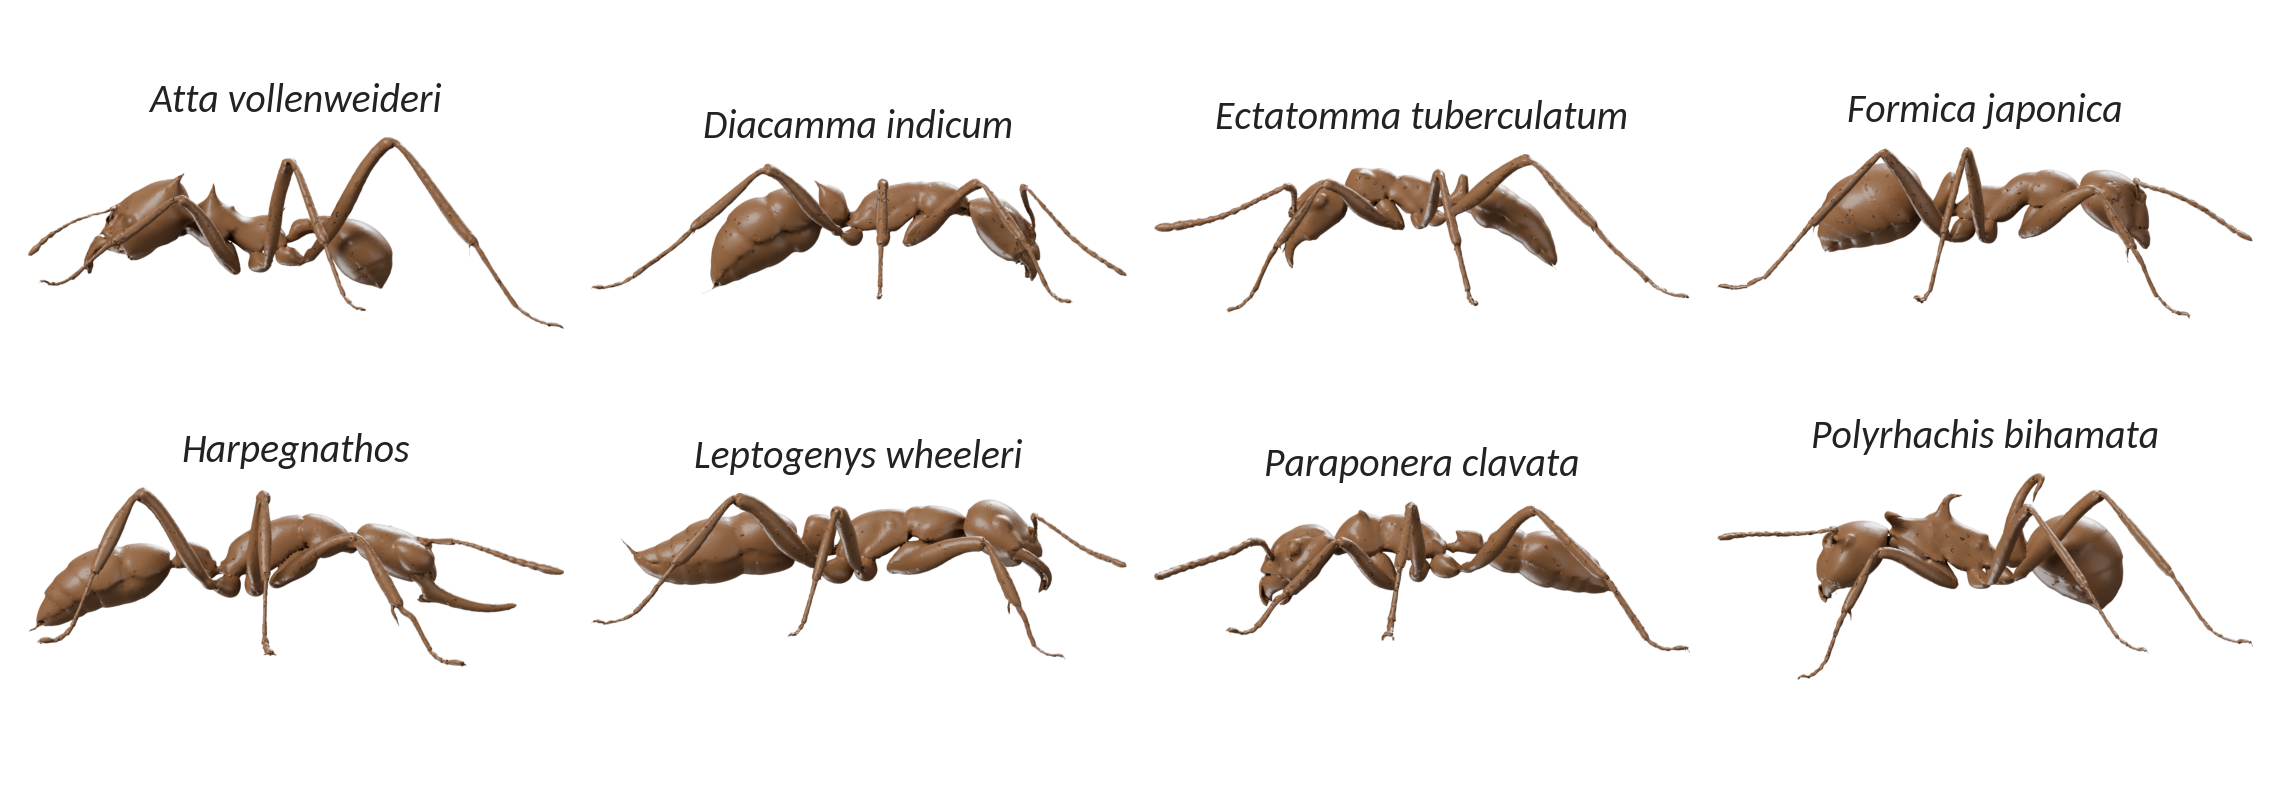
\includegraphics[width=0.62\linewidth]{figures/fig_corpus_gallery.png}
\caption[Diversity of the curated corpus]{Eight genera from the curated corpus of clean
scans, rendered under identical conditions: the shared representation has to accommodate
differences in body plan, proportions, posture and articulation.}
\label{fig:corpus}
\end{figure}

The value of the work is therefore not only the fitted mesh. It is an understanding of how
to construct the representation, how to fit it, where the fitting can fail, and how to
establish what its parameters mean. The question that started the project was how to bring
many different meshes into one shared representation; the harder question it leads to is
what that representation can be trusted to mean. Once that is established, the value extends
beyond reconstruction: it becomes a way of making morphology measurable.


\bibliography{bib/references}

\clearpage
% Back cover (quatri\`eme de couverture), no page number
\thispagestyle{empty}
\vspace*{0.26\textheight}
\begin{center}

\includegraphics[height=1.4cm]{figures/logos/juelich_blue.png}\hspace{1.6cm}
\includegraphics[height=1.4cm]{figures/logos/coc_dark.png}\par
\vspace{1.4cm}
{\fontsize{20}{25}\selectfont\bfseries\color{accent} Mesh Registration from\\ Scan-Derived 3D Data\par}
\vspace{0.6cm}
{\large\itshape Correspondence and optimization in articulated parametric models of insects\par}
\vspace{1.2cm}
\textcolor{rule}{\rule{0.4\linewidth}{0.6pt}}\par
\vspace{0.8cm}
Khaoula Jellal\par
Internship report, 1 July -- 25 September 2026\par
\vspace{0.4cm}
Forschungszentrum J\"ulich GmbH, Institute for Advanced Simulation, IAS-7\par
College of Computing -- UM6P\par
\end{center}


\end{document}
